% Apéndices y anexos. Este archivo se incorpora una sola vez desde main.tex.
% La clase article utiliza section como unidad de apéndice; por ello A y B corresponden a los manuales.
\appendix
\renewcommand{\thesection}{\Alph{section}}
\renewcommand{\thefigure}{\thesection\arabic{figure}}
\renewcommand{\thetable}{\thesection\arabic{table}}
\setcounter{section}{0}
\setcounter{figure}{0}
\setcounter{table}{0}

% Encabezado general solicitado por la guía antes del primer manual.
% Se presenta como página independiente y no se incorpora al índice general.
\clearpage
\thispagestyle{cuerpo}
\begin{center}
\vspace*{3cm}
{\Large\bfseries Apendices\par}
\vspace{1cm}
{\normalsize Material complementario de la tesis\par}
\end{center}
\clearpage

\section{Anexos}\label{anexos}

\subsection{Formato de Encuesta}\label{formato-de-encuesta}

\begin{figure}[H]
    \begin{flushleft}
        \textbf{Figura Anexo C1}\\
        \emph{Formato Cuestionario en Blanco 1}
    \end{flushleft}
    \vspace{0.1cm}
    \centering
    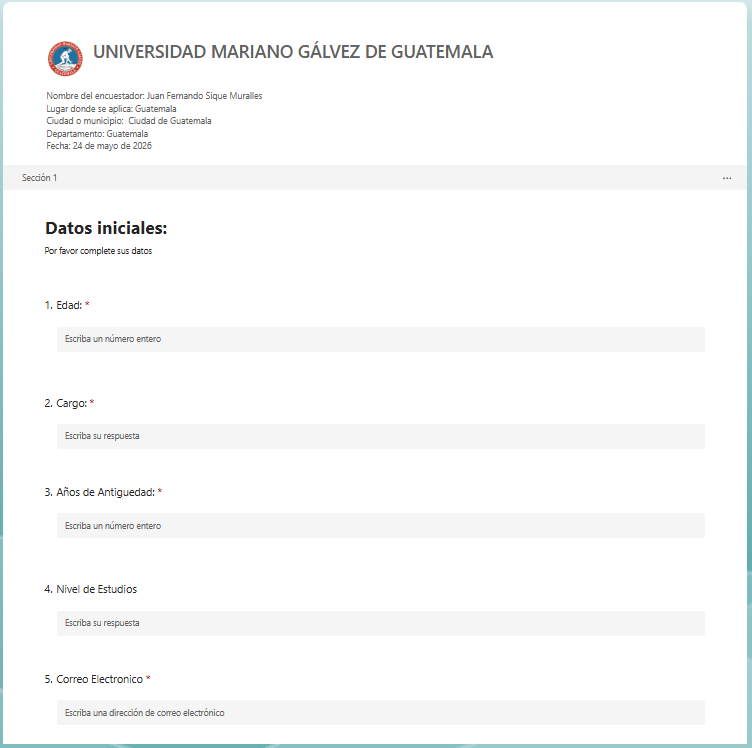
\includegraphics[width=\textwidth]{./imagenes/image8.png}
\end{figure}

\begin{figure}[H]
    \begin{flushleft}
        \textbf{Figura Anexo C2}\\
        \emph{Formato cuestionario en Blanco 2}
    \end{flushleft}
    \vspace{0.1cm}
    \centering
    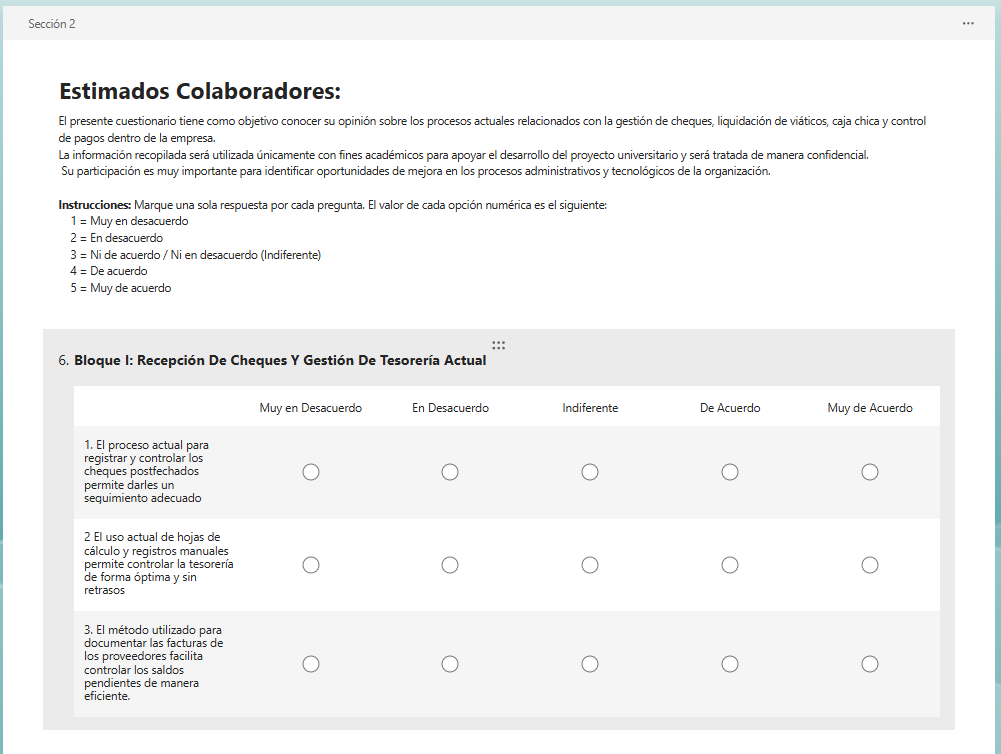
\includegraphics[width=\textwidth]{./imagenes/image9.png}
\end{figure}

\begin{figure}[H]
    \begin{flushleft}
        \textbf{Figura Anexo C3}\\
        \emph{Formato cuestionario en Blanco 3}
    \end{flushleft}
    \vspace{0.1cm}
    \centering
    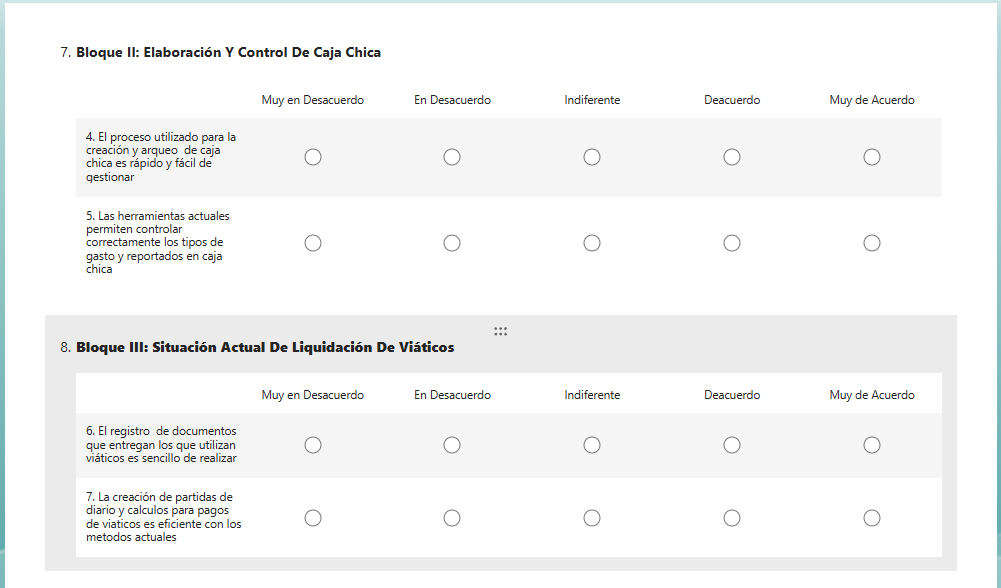
\includegraphics[width=\textwidth]{./imagenes/image10.png}
\end{figure}

\begin{figure}[H]
    \begin{flushleft}
        \textbf{Figura Anexo C4}\\
        \emph{Formato cuestionario en Blanco 4}
    \end{flushleft}
    \vspace{0.1cm}
    \centering
    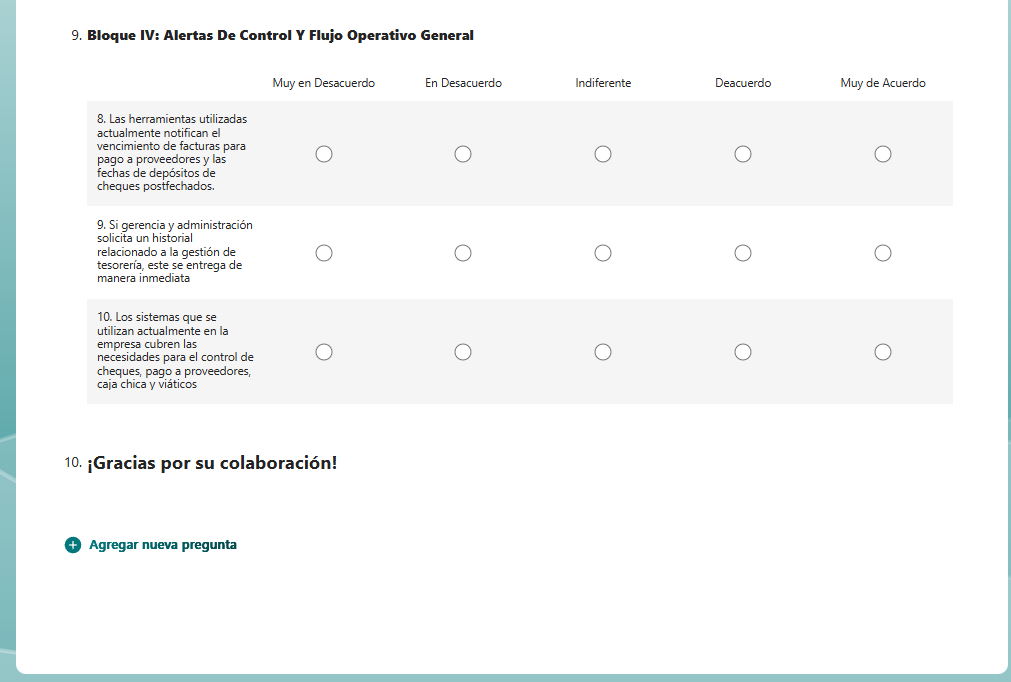
\includegraphics[width=\textwidth]{./imagenes/image11.png}
\end{figure}

\subsection{Muestra de Aplicación}\label{muestra-de-aplicacion}

\begin{figure}[H]
    \begin{flushleft}
        \textbf{Figura Anexo C5}\\
        \emph{Formato cuestionario 1 lleno 1}
    \end{flushleft}
    \vspace{0.1cm}
    \centering
    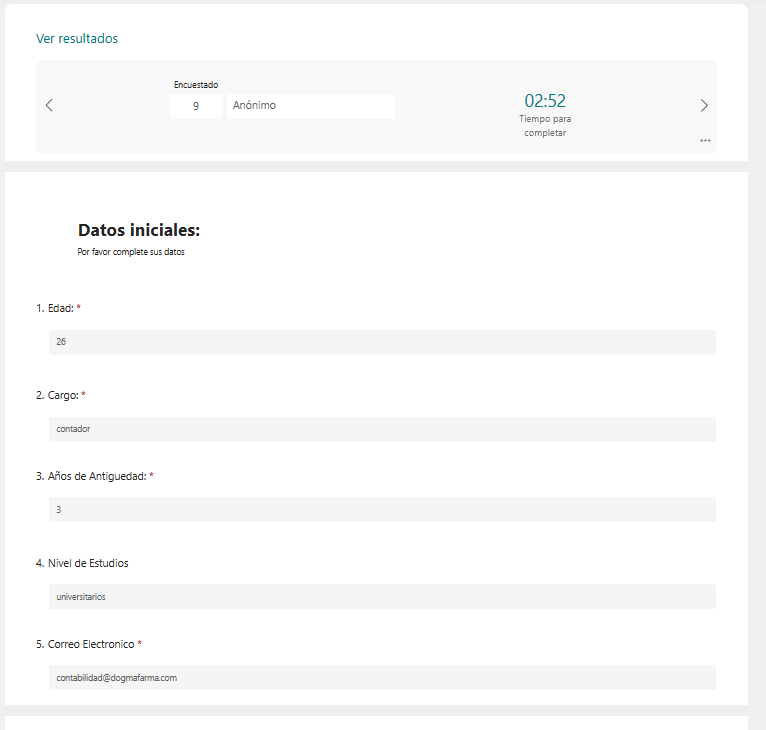
\includegraphics[width=\textwidth]{./imagenes/image12.png}
\end{figure}

\begin{figure}[H]
    \begin{flushleft}
        \textbf{Figura Anexo C6}\\
        \emph{Formato cuestionario 1 lleno 2}
    \end{flushleft}
    \vspace{0.1cm}
    \centering
    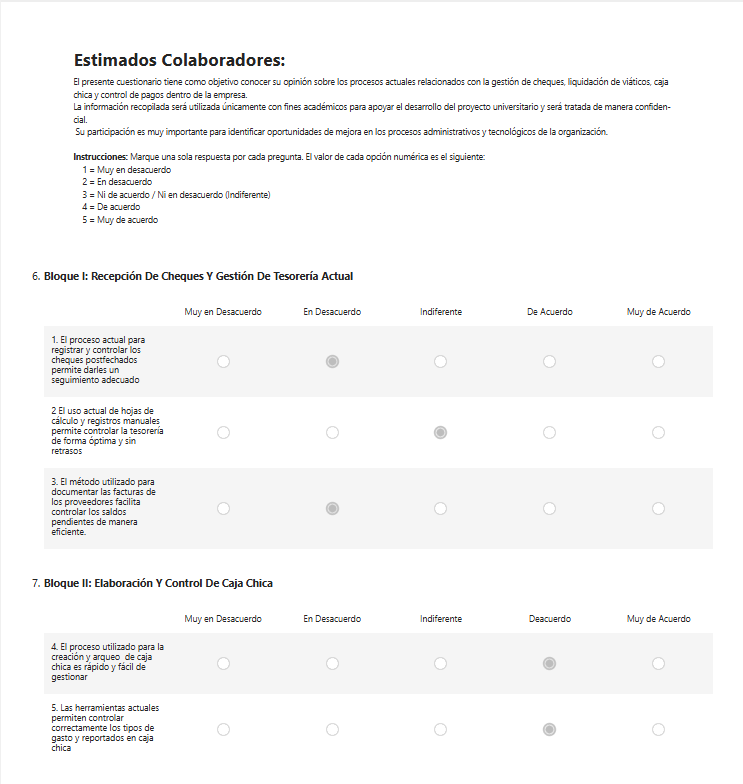
\includegraphics[width=\textwidth]{./imagenes/image13.png}
\end{figure}

\begin{figure}[H]
    \begin{flushleft}
        \textbf{Figura Anexo C7}\\
        \emph{Formato cuestionario 1 lleno 3}
    \end{flushleft}
    \vspace{0.1cm}
    \centering
    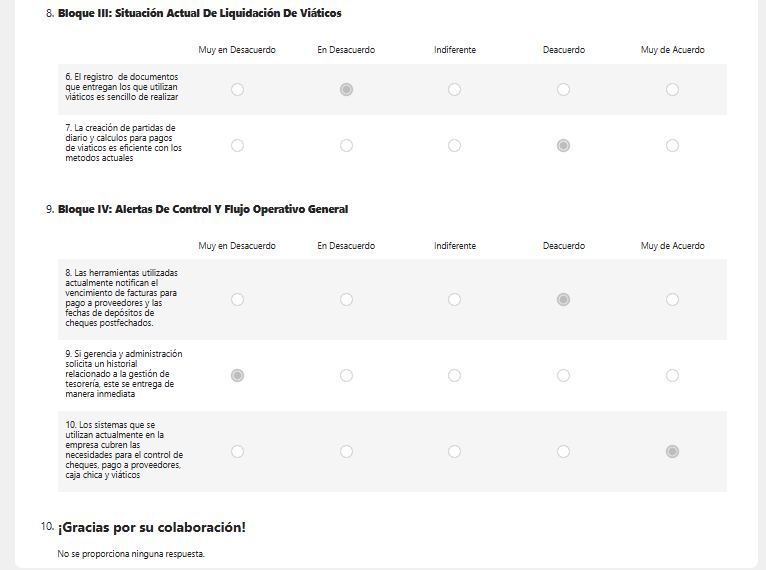
\includegraphics[width=\textwidth]{./imagenes/image14.png}
\end{figure}

\begin{figure}[H]
    \begin{flushleft}
        \textbf{Figura Anexo C8}\\
        \emph{Formato cuestionario 2 lleno 1}
    \end{flushleft}
    \vspace{0.1cm}
    \centering
    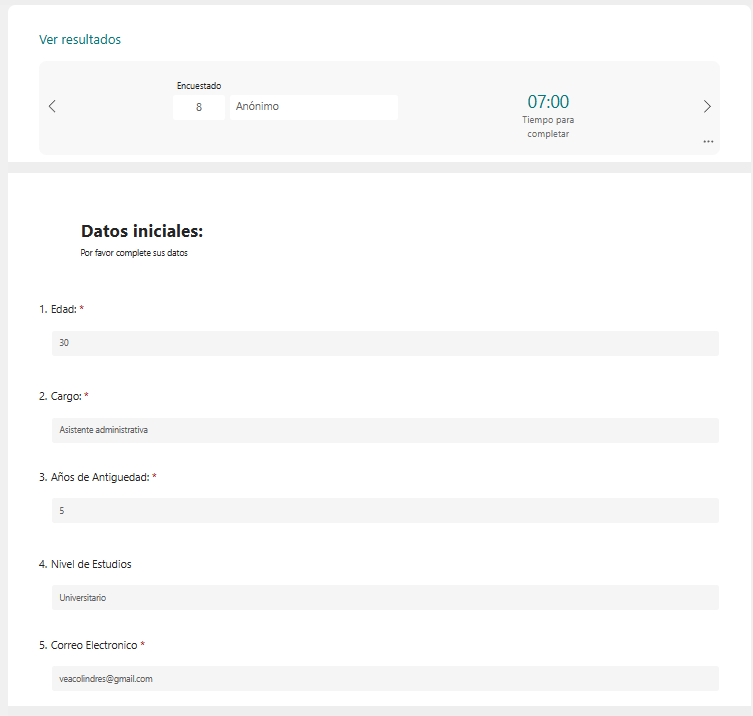
\includegraphics[width=\textwidth]{./imagenes/image15.png}
\end{figure}

\begin{figure}[H]
    \begin{flushleft}
        \textbf{Figura Anexo C9}\\
        \emph{Formato cuestionario 2 lleno 2}
    \end{flushleft}
    \vspace{0.1cm}
    \centering
    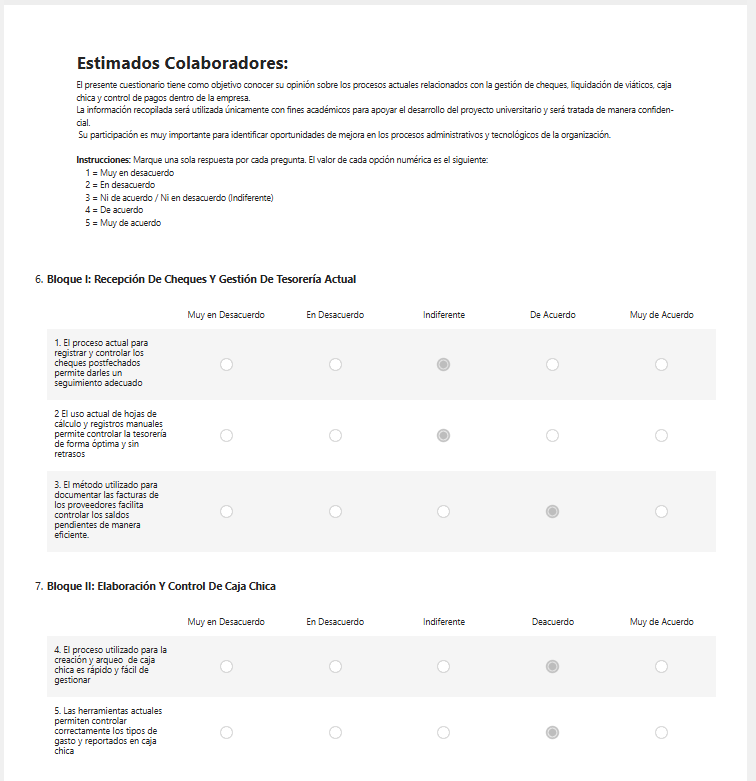
\includegraphics[width=\textwidth]{./imagenes/image16.png}
\end{figure}

\begin{figure}[H]
    \begin{flushleft}
        \textbf{Figura Anexo C10}\\
        \emph{Formato cuestionario 2 lleno 3}
    \end{flushleft}
    \vspace{0.1cm}
    \centering
    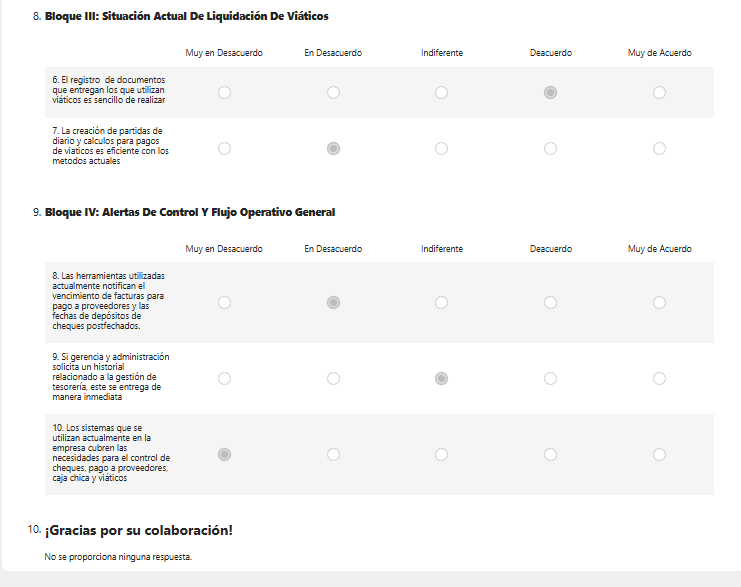
\includegraphics[width=\textwidth]{./imagenes/image17.png}
\end{figure}

\subsection{Interpretación de Escala de Likert}\label{interpretacion-de-escala-de-likert}

\begin{figure}[H]
    \begin{flushleft}
        \textbf{Figura Anexo C11}\\
        \emph{Resultado de la Escala de Likert}
    \end{flushleft}
    \vspace{0.1cm}
    \centering
    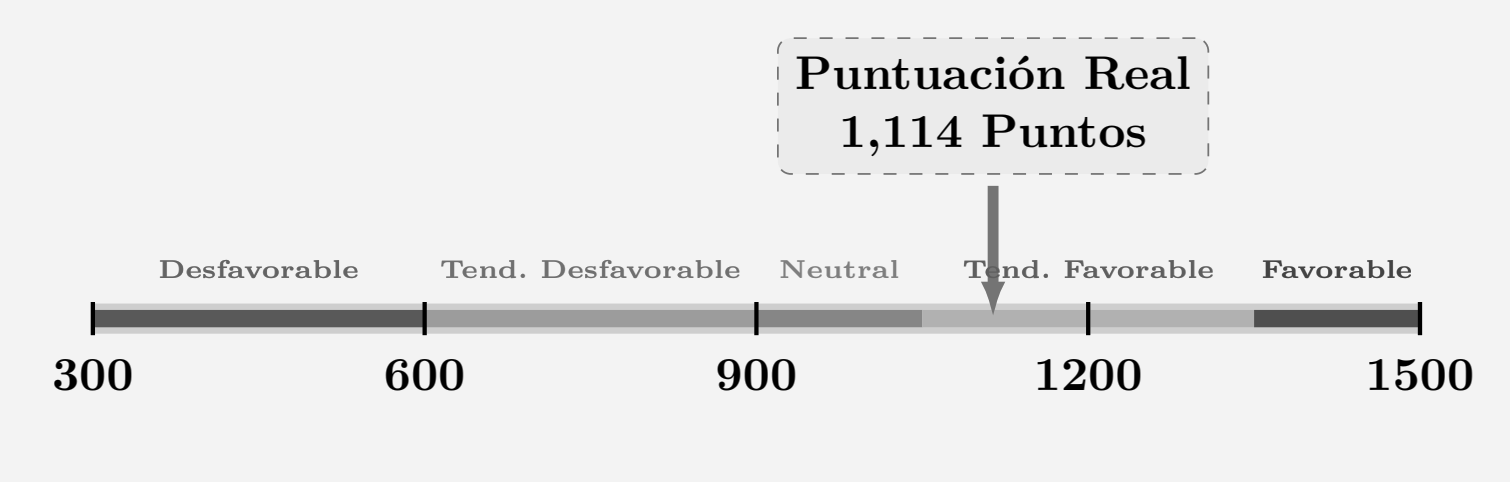
\includegraphics[width=\textwidth]{./imagenes/image18.png}
\end{figure}

\begin{figure}[H]
    \begin{flushleft}
        \textbf{Figura Anexo C12}\\
        \emph{Bloque I}
    \end{flushleft}
    \vspace{0.1cm}
    \centering
    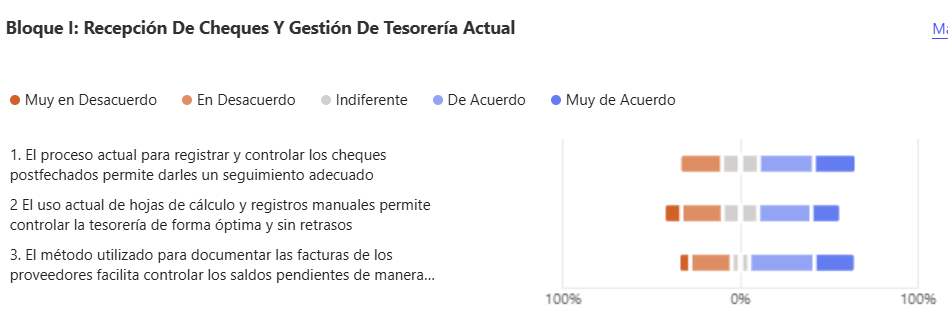
\includegraphics[width=\textwidth]{./imagenes/image19.png}
\end{figure}

\begin{table}[H]
\small
\begin{flushleft}
    \textbf{Tabla Anexo C1}\\[0.2cm]
    \emph{Bloque I (Porcentajes Tres preguntas)}
\end{flushleft}
\renewcommand{\arraystretch}{1.0}
\centering
\begin{tabular}{
    >{\raggedright\arraybackslash}p{2.6cm} 
    >{\raggedright\arraybackslash}p{1.6cm} 
    >{\raggedright\arraybackslash}p{1.6cm} 
    >{\raggedright\arraybackslash}p{1.6cm} 
    >{\raggedright\arraybackslash}p{2.0cm} 
    >{\raggedright\arraybackslash}p{2.3cm} 
    >{\raggedright\arraybackslash}p{1.8cm}
}
\toprule
\textbf{Preguntas} & \textbf{Muy de\newline Acuerdo} & \textbf{De\newline Acuerdo} & \textbf{Indiferente} & \textbf{En\newline Desacuerdo} & \textbf{Muy en\newline Desacuerdo} & \textbf{Sin\newline Respuesta} \\
\midrule
P.1 & 7 & 9 & 6 & 7 & 0 & 1 \\
P.2 & 5 & 9 & 6 & 7 & 3 & 0 \\
P.3 & 7 & 11 & 3 & 7 & 2 & 0 \\
\midrule
\textbf{Suma Bloque} & \textbf{19} & \textbf{29} & \textbf{15} & \textbf{21} & \textbf{5} & \textbf{1} \\
\textbf{Total (\%)} & \textbf{21.1\%} & \textbf{32.2\%} & \textbf{16.7\%} & \textbf{23.3\%} & \textbf{5.6\%} & \textbf{1.1\%} \\
\bottomrule
\end{tabular}
\end{table}

\begin{figure}[H]
    \begin{flushleft}
        \textbf{Figura Anexo C13}\\
        \emph{Bloque II}
    \end{flushleft}
    \vspace{0.1cm}
    \centering
    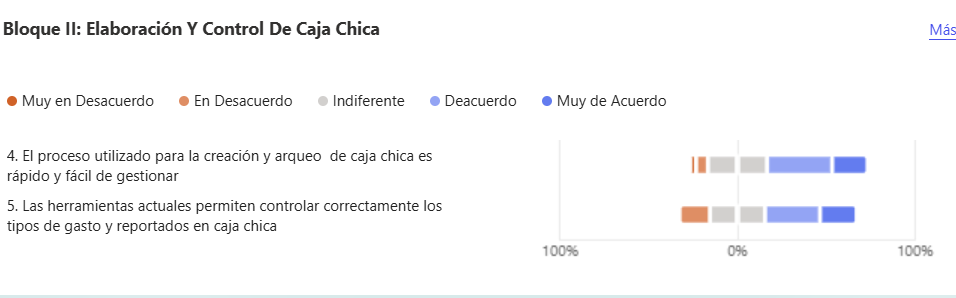
\includegraphics[width=\textwidth]{./imagenes/image20.png}
\end{figure}

\begin{table}[H]
\small
\begin{flushleft}
    \textbf{Tabla Anexo C2}\\[0.2cm]
    \emph{Bloque II (Porcentajes dos preguntas)}
\end{flushleft}
\renewcommand{\arraystretch}{1.0}
\centering
\begin{tabular}{
    >{\raggedright\arraybackslash}p{2.6cm} 
    >{\raggedright\arraybackslash}p{1.6cm} 
    >{\raggedright\arraybackslash}p{1.6cm} 
    >{\raggedright\arraybackslash}p{1.6cm} 
    >{\raggedright\arraybackslash}p{2.0cm} 
    >{\raggedright\arraybackslash}p{2.3cm} 
    >{\raggedright\arraybackslash}p{1.8cm}
}
\toprule
\textbf{Preguntas} & \textbf{Muy de\newline Acuerdo} & \textbf{De\newline Acuerdo} & \textbf{Indiferente} & \textbf{En\newline Desacuerdo} & \textbf{Muy en\newline Desacuerdo} & \textbf{Sin\newline Respuesta} \\
\midrule
P.4 & 6 & 11 & 10 & 2 & 1 & 0 \\
P.5 & 6 & 9 & 9 & 5 & 0 & 1 \\
\midrule
\textbf{Suma Bloque} & \textbf{12} & \textbf{20} & \textbf{19} & \textbf{7} & \textbf{1} & \textbf{1} \\
\textbf{Total (\%)} & \textbf{20.0\%} & \textbf{33.3\%} & \textbf{31.7\%} & \textbf{11.7\%} & \textbf{1.7\%} & \textbf{1.6\%} \\
\bottomrule
\end{tabular}
\end{table}

\begin{figure}[H]
    \begin{flushleft}
        \textbf{Figura Anexo C14}\\
        \emph{Bloque III}
    \end{flushleft}
    \vspace{0.1cm}
    \centering
    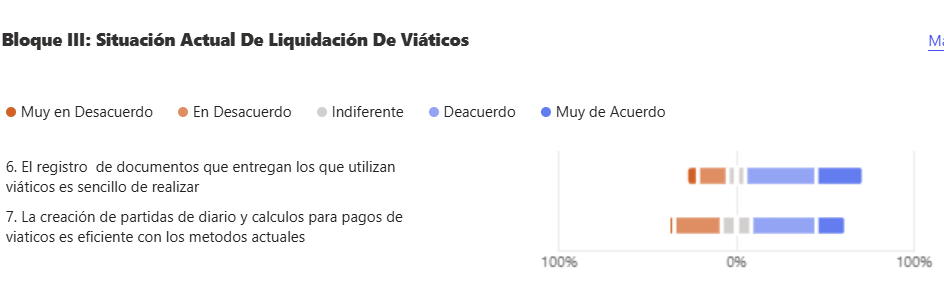
\includegraphics[width=\textwidth]{./imagenes/image21.png}
\end{figure}

\begin{table}[H]
\small
\begin{flushleft}
    \textbf{Tabla Anexo C3}\\[0.2cm]
    \emph{Bloque III (Porcentajes Dos preguntas)}
\end{flushleft}
\renewcommand{\arraystretch}{1.0}
\centering
\begin{tabular}{
    >{\raggedright\arraybackslash}p{2.6cm} 
    >{\raggedright\arraybackslash}p{1.6cm} 
    >{\raggedright\arraybackslash}p{1.6cm} 
    >{\raggedright\arraybackslash}p{1.6cm} 
    >{\raggedright\arraybackslash}p{2.0cm} 
    >{\raggedright\arraybackslash}p{2.3cm} 
    >{\raggedright\arraybackslash}p{1.8cm}
}
\toprule
\textbf{Preguntas} & \textbf{Muy de\newline Acuerdo} & \textbf{De\newline Acuerdo} & \textbf{Indiferente} & \textbf{En\newline Desacuerdo} & \textbf{Muy en\newline Desacuerdo} & \textbf{Sin\newline Respuesta} \\
\midrule
P.6 & 8 & 12 & 3 & 5 & 2 & 0 \\
P.7 & 5 & 11 & 5 & 8 & 1 & 0 \\
\midrule
\textbf{Suma Bloque} & \textbf{13} & \textbf{23} & \textbf{8} & \textbf{13} & \textbf{3} & \textbf{0} \\
\textbf{Total (\%)} & \textbf{21.7\%} & \textbf{38.3\%} & \textbf{13.3\%} & \textbf{21.7\%} & \textbf{5.0\%} & \textbf{0.0\%} \\
\bottomrule
\end{tabular}
\end{table}

\begin{figure}[H]
\begin{flushleft}
    \textbf{Figura Anexo C15}\\
    \emph{Bloque IV}
\end{flushleft}
\vspace{0.1cm}
\centering
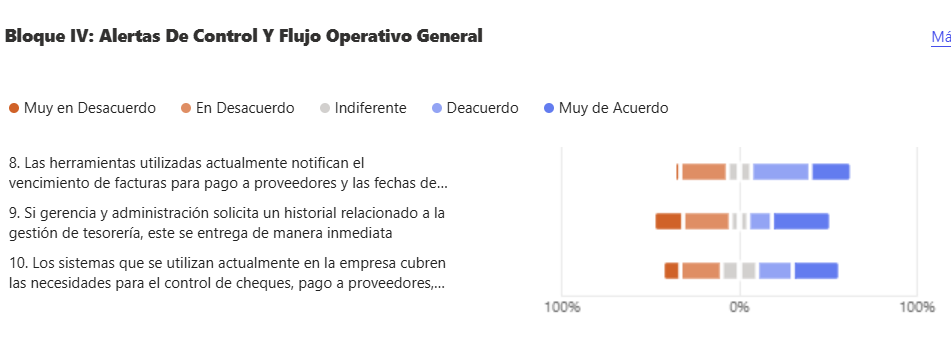
\includegraphics[width=\textwidth]{./imagenes/image22.png}
\end{figure}

\begin{table}[H]
\small
\begin{flushleft}
    \textbf{Tabla Anexo C4}\\[0.2cm]
    \emph{Bloque IV (Porcentajes Tres preguntas)}
\end{flushleft}
\renewcommand{\arraystretch}{1.0}
\centering
\begin{tabular}{
    >{\raggedright\arraybackslash}p{2.6cm} 
    >{\raggedright\arraybackslash}p{1.6cm} 
    >{\raggedright\arraybackslash}p{1.6cm} 
    >{\raggedright\arraybackslash}p{1.6cm} 
    >{\raggedright\arraybackslash}p{2.0cm} 
    >{\raggedright\arraybackslash}p{2.3cm} 
    >{\raggedright\arraybackslash}p{1.8cm}
}
\toprule
\textbf{Preguntas} & \textbf{Muy de\newline Acuerdo} & \textbf{De\newline Acuerdo} & \textbf{Indiferente} & \textbf{En\newline Desacuerdo} & \textbf{Muy en\newline Desacuerdo} & \textbf{Sin\newline Respuesta} \\
\midrule
P.8 & 7 & 10 & 4 & 8 & 1 & 0 \\
P.9 & 10 & 4 & 3 & 8 & 5 & 0 \\
P.10 & 8 & 6 & 6 & 7 & 3 & 0 \\
\midrule
\textbf{Suma Bloque} & \textbf{25} & \textbf{20} & \textbf{13} & \textbf{23} & \textbf{9} & \textbf{0} \\
\textbf{Total (\%)} & \textbf{27.8\%} & \textbf{22.2\%} & \textbf{14.4\%} & \textbf{25.6\%} & \textbf{10.0\%} & \textbf{0.0\%} \\
\bottomrule
\end{tabular}
\end{table}
\captionsetup{list=true}

% Los manuales y anexos conservan sus captions, pero no se incorporan
% a los índices generales de figuras y tablas de la tesis.
\captionsetup{list=false}
% Manual de Usuario del Sistema Web de gestión contable.
% Este archivo se incorpora directamente desde main.tex como Apéndice A.
% Las capturas anotadas utilizan numeración correlativa y pasos operativos.

\newpage
\section*{Apéndice}\label{Apendice}
\addcontentsline{toc}{section}{Apéndice}

\appendix
% El Manual de Usuario corresponde al Apéndice A.
\setcounter{section}{1}
\renewcommand{\thesection}{\Alph{section}}
\renewcommand{\thesubsection}{\thesection.\arabic{subsection}}
\renewcommand{\thefigure}{\thesection\arabic{figure}}
\renewcommand{\thetable}{\thesection\arabic{table}}
\setcounter{figure}{0}
\setcounter{table}{0}
\setcounter{tocdepth}{0}
\captionsetup{list=false}
\pagestyle{cuerpo}

\setcounter{subsection}{0}
\subsection{Manual de Usuario}\label{ap:Manual-de-Usuario}
\phantomsection
\addcontentsline{toc}{section}{Apéndice A Manual de Usuario}
\begin{center}
\vspace*{2cm}
{\Large\textbf{APÉNDICE A}}\par
\vspace{1.5cm}
{\Large\textbf{MANUAL DE USUARIO}}\par
\vspace{0.8cm}
{\large Sistema Web de gestión contable}\par
\vspace{2cm}
\begin{minipage}{0.82\textwidth}
\centering
Guía para el ingreso al sistema, consulta y registro de facturas FEL/SAT, cheques posfechados, caja chica, viáticos, proveedores, calendario, nomenclatura contable y reportes.
\end{minipage}
\vfill
Documento complementario del trabajo de graduación\par
\end{center}


\setlength{\parindent}{1.27cm}
\setlength{\parskip}{0pt}
\setstretch{2.0}

\subsubsection{Introducción}
Este manual orienta al usuario final en el uso del Sistema Web para el control de facturas FEL/SAT, cheques posfechados, caja chica, viáticos, proveedores, nomenclatura contable, calendario y reportes. Cada pantalla se presenta con una captura del prototipo funcional y una versión anotada. Los números rojos de la imagen corresponden directamente a los pasos descritos debajo de ella.

Los datos que aparecen en las figuras son demostrativos. El usuario debe aplicar, además, las políticas internas de autorización, revisión y resguardo de documentos contables.

\subsubsection{Requisitos del sistema}
El correcto funcionamiento y uso del Sistema Web depende de que el equipo del usuario tenga acceso a la red institucional, un navegador actualizado y las credenciales autorizadas. Los requisitos se organizan entre el lado del cliente, utilizado por el personal operativo, y el lado del servidor, administrado por el personal técnico.

\paragraph{Requisitos del lado del cliente}
El lado del cliente corresponde al equipo desde el cual el usuario consulta y registra información. El sistema debe ejecutarse en un navegador compatible con aplicaciones web modernas y con acceso habilitado a la dirección institucional de la plataforma.

\paragraph{Infraestructura de software del cliente}
\begin{itemize}
\item Navegador web actualizado, como Google Chrome, Mozilla Firefox, Microsoft Edge o Safari.
\item JavaScript habilitado para permitir la ejecución de la interfaz desarrollada en Angular.
\item Cookies y almacenamiento local habilitados cuando sean necesarios para conservar la sesión autorizada.
\item Sistema operativo de escritorio compatible con el navegador instalado.
\item Cuenta de usuario activa, con el perfil y los permisos asignados por la organización.
\end{itemize}

\paragraph{Conectividad del cliente}
El equipo debe mantener una conexión estable con la red institucional o con el servicio autorizado para acceder al sistema. Si la conexión se interrumpe durante un registro, el usuario debe verificar si la operación fue guardada antes de repetirla, con el fin de evitar duplicidad de documentos o movimientos.

\paragraph{Requisitos del lado del servidor}
El lado del servidor debe mantener disponibles los servicios del frontend Angular, el backend desarrollado en Python/FastAPI y la base de datos PostgreSQL. La configuración debe separar las credenciales y variables de los ambientes de desarrollo, pruebas y producción.

\paragraph{Entorno de software del servidor}
\begin{itemize}
\item Sistema operativo de servidor compatible con Python, Angular y PostgreSQL.
\item Runtime de Python y dependencias del backend documentados en el archivo de configuración del proyecto.
\item Servicio backend Python/FastAPI para autenticación, validación y reglas de negocio.
\item Servicio de publicación del frontend Angular con conexión segura al backend.
\item PostgreSQL para almacenar usuarios, facturas, cheques, movimientos, cuentas, proveedores y reportes.
\item Certificado SSL/TLS y configuración de acceso restringido para proteger la comunicación.
\end{itemize}

\paragraph{Dimensionamiento de referencia}
La siguiente tabla presenta una referencia mínima para el ambiente del servidor. El dimensionamiento definitivo debe revisarse según el número de usuarios, el volumen de facturas y las políticas de infraestructura de la organización.

\begin{longtable}{p{4.0cm}p{4.3cm}p{4.3cm}}
\caption{Requisitos de infraestructura de referencia}\label{tab:A_requisitos_sistema}\\
\toprule
\textbf{Componente} & \textbf{Configuración mínima} & \textbf{Configuración recomendada}\\
\midrule
Procesador & 1 núcleo virtual de 64 bits & 2 núcleos virtuales o físicos dedicados\\
Memoria RAM & 2 GB disponibles & 4 GB o superior\\
Almacenamiento & 10 GB libres para aplicación, logs y configuración & 30 GB libres en unidad de estado sólido\\
Base de datos & PostgreSQL configurado con respaldo periódico & PostgreSQL con almacenamiento separado y monitoreo\\
Red & Conexión estable para atender las solicitudes del sistema & Enlace institucional con monitoreo de disponibilidad\\
Respaldo & Copia periódica de la base de datos & Copia automática externa y prueba de restauración\\
\bottomrule
\end{longtable}

\textit{Nota.} Los valores son de referencia para la instalación y deben ajustarse al crecimiento de usuarios, documentos y registros contables.

\subsubsection{Acceso al sistema}
Abra el navegador, escriba la dirección web proporcionada por el administrador y espere a que se muestre la pantalla de acceso.

\subsubsection{Ingreso al sistema}
En la sección de acceso, siga los pasos ilustrados en la captura anotada para ingresar al sistema.

\subsubsection{Descripción general del sistema}
El Sistema Web organiza en un menú lateral los módulos de Facturas FEL/SAT, Cheques, Caja chica, Viáticos, Proveedores, Calendario, Nomenclatura y Reportes. El Panel principal presenta alertas e indicadores del período activo, mientras que cada módulo permite registrar, consultar y dar seguimiento a las operaciones autorizadas.

\begin{figure}[H]
    \centering
    \caption{Pantalla de acceso con anotaciones numeradas.}
    \label{fig:manual_usuario_pantalla_01_login_anotada}
    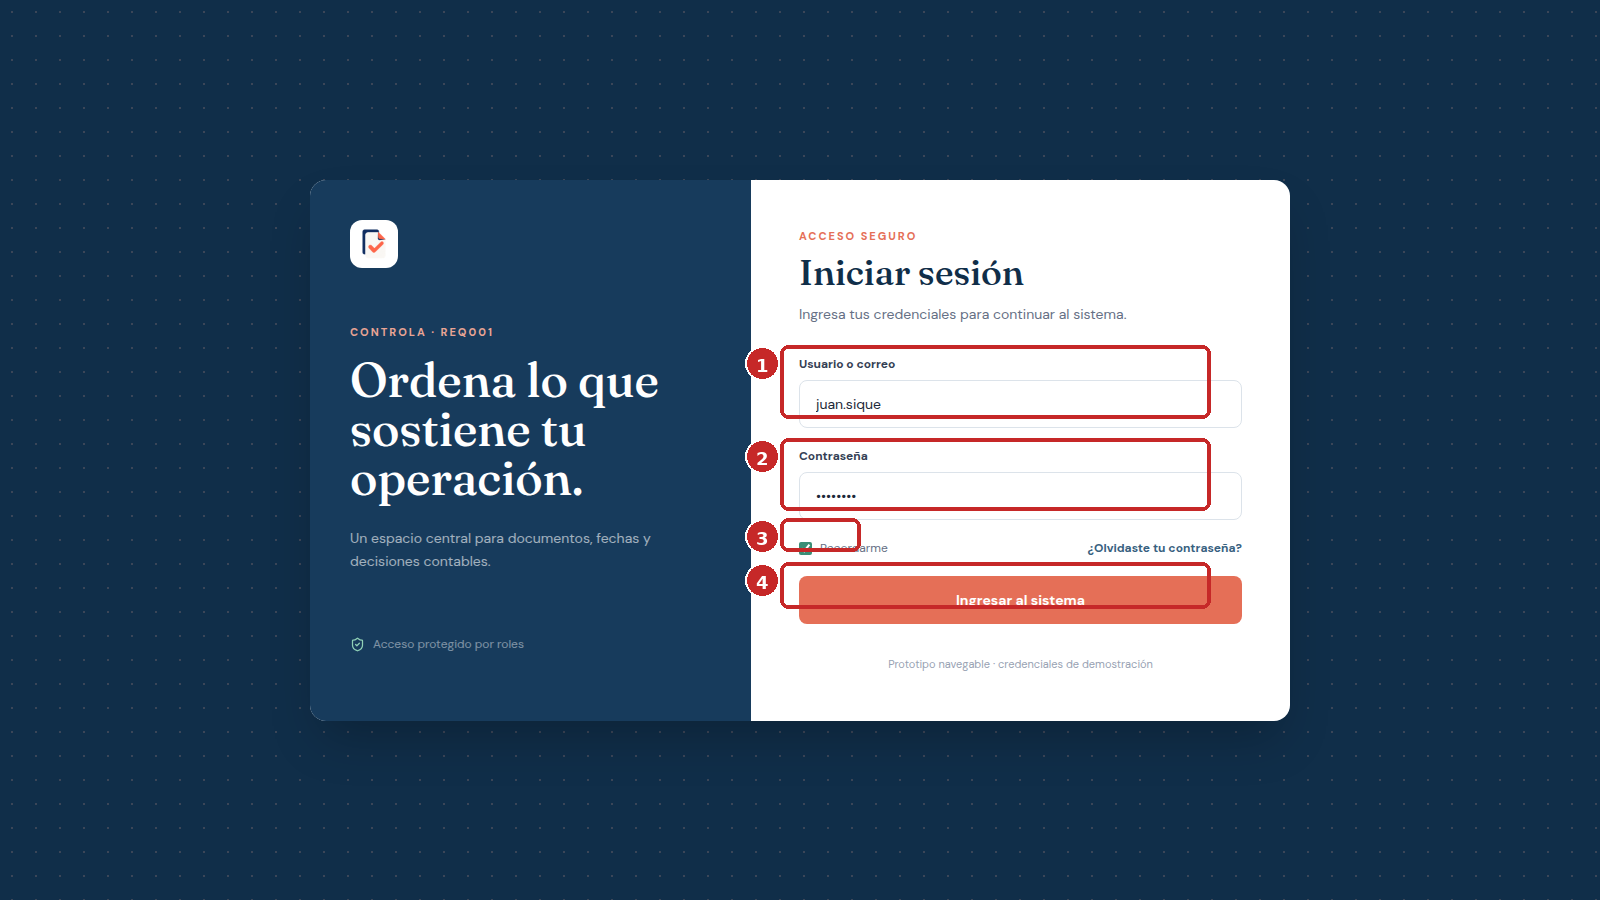
\includegraphics[width=0.92\linewidth]{capturas_reales/anotadas/pantalla_01_login_anotada.png}
    \caption*{Nota. Elaboración propia a partir del prototipo funcional.}
\end{figure}

\begin{enumerate}
\item Haga clic en el campo de usuario y escriba el nombre de usuario o correo electrónico habilitado.
\item Haga clic en el campo de contraseña y escriba la clave sin agregar espacios al inicio o al final.
\item Haga clic en la casilla ``Recordarme'' únicamente si el equipo es institucional y cumple las políticas de seguridad.
\item Haga clic en ``Ingresar al sistema''.
\item El sistema validará las credenciales y mostrará el Panel principal. Si aparece un mensaje de error, revise los datos y solicite apoyo al administrador cuando sea necesario.
\end{enumerate}

\subsubsection{Uso del sistema}
Las instrucciones siguientes describen las operaciones principales del sistema mediante capturas anotadas. Realice cada paso en el orden indicado y verifique el mensaje mostrado antes de continuar.

\subsubsection{Panel principal}
El Panel principal concentra la información operativa del período contable seleccionado.

\begin{figure}[H]
    \centering
    \caption{Panel principal con anotaciones numeradas.}
    \label{fig:manual_usuario_pantalla_02_dashboard_anotada}
    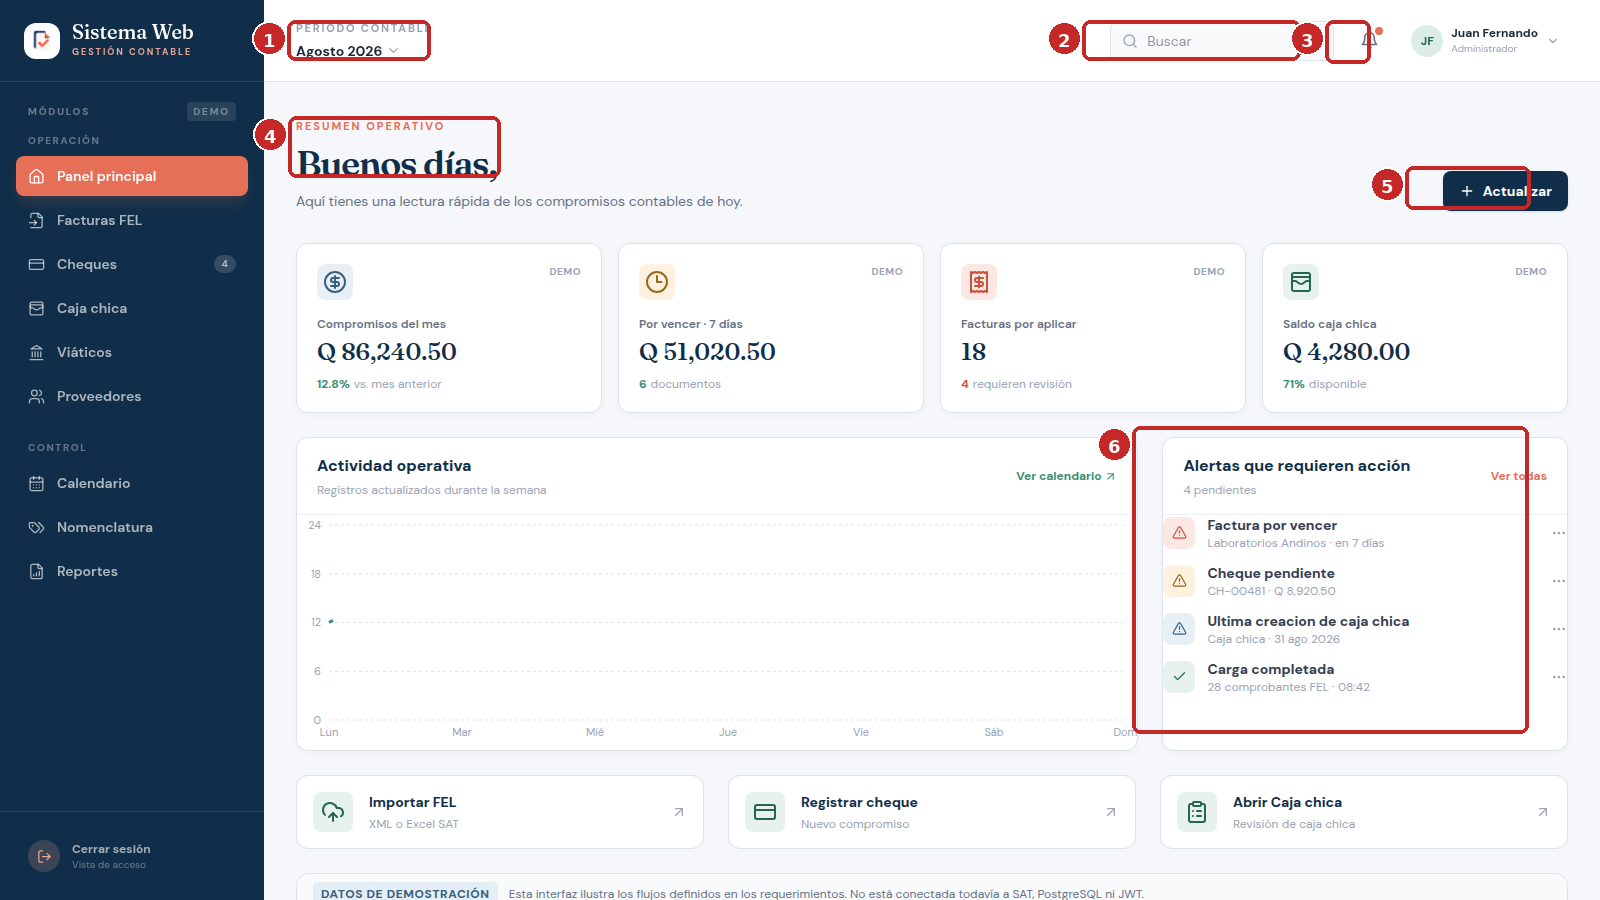
\includegraphics[width=0.92\linewidth]{capturas_reales/anotadas/pantalla_02_dashboard_anotada.png}
    \caption*{Nota. Elaboración propia a partir del prototipo funcional.}
\end{figure}

\begin{enumerate}
\item Revise el período contable activo.
\item Haga clic en ``Buscar'' y escriba el criterio de consulta.
\item Revise las alertas operativas pendientes.
\item Revise los indicadores de compromisos, vencimientos, facturas y saldo de Caja chica.
\item Haga clic en ``Actualizar'' para refrescar la información mostrada.
\item Revise las alertas y seleccione la que requiera atención.
\item Para cambiar de módulo, seleccione una opción del menú lateral, por ejemplo ``Facturas FEL'', ``Cheques'', ``Caja chica'', ``Viáticos'', ``Proveedores'', ``Calendario'', ``Nomenclatura'' o ``Reportes''.
\end{enumerate}

\subsubsection{Facturas FEL/SAT}
Este módulo permite importar archivos XML o Excel descargados del portal SAT, revisar comprobantes y detectar duplicados o documentos que requieren revisión.

\begin{figure}[H]
    \centering
    \caption{Módulo de Facturas FEL/SAT con anotaciones numeradas.}
    \label{fig:manual_usuario_pantalla_03_facturas_fel_anotada}
    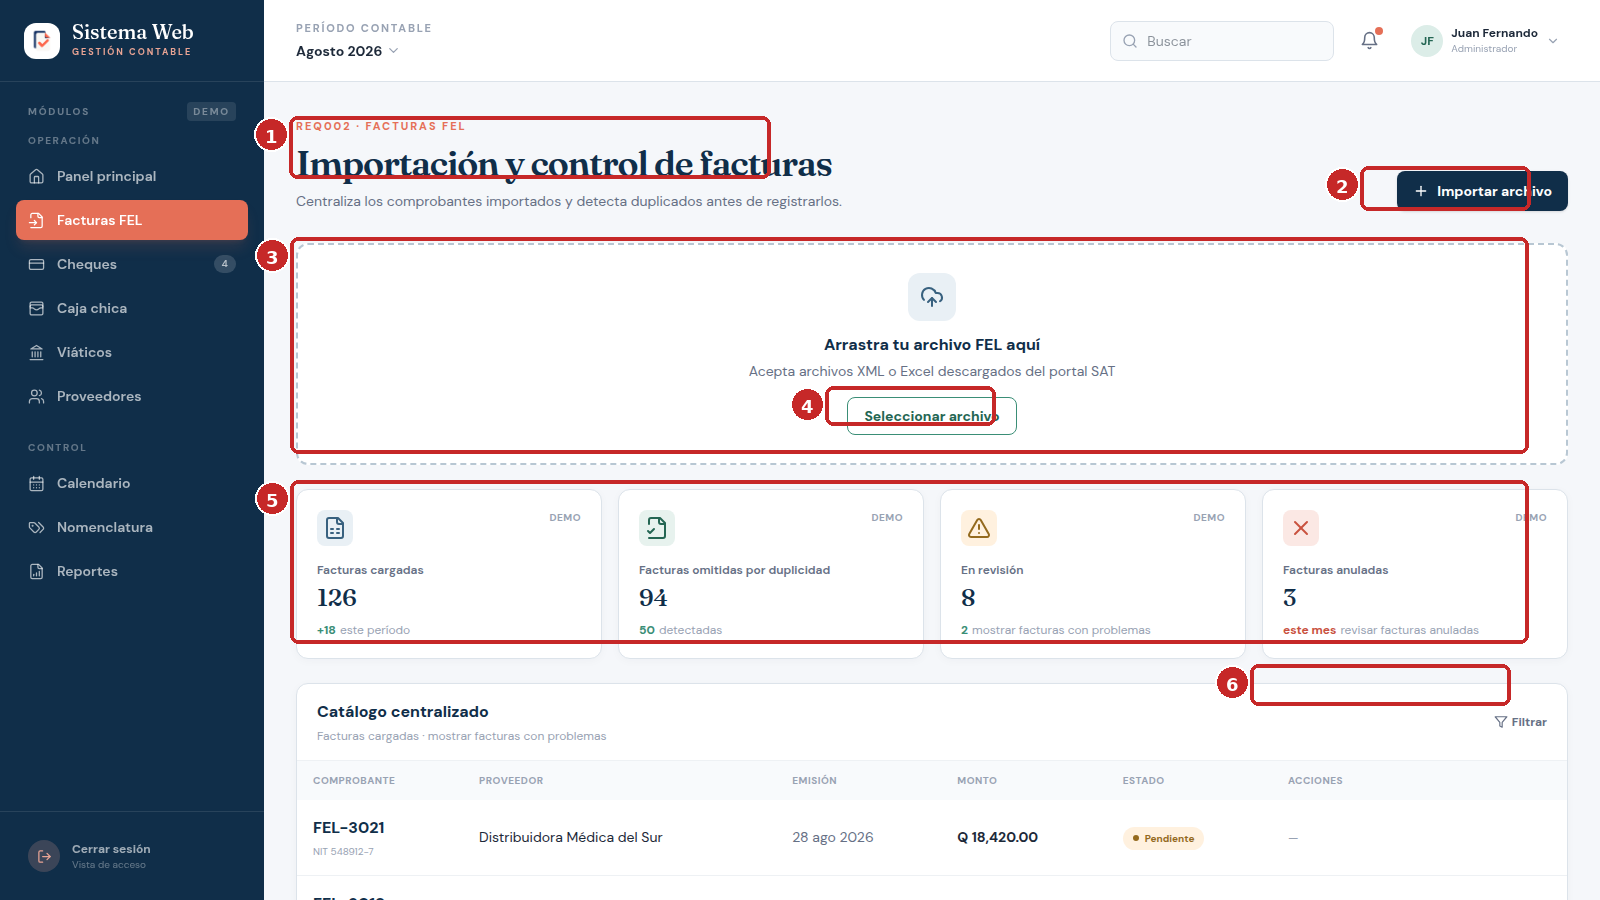
\includegraphics[width=0.92\linewidth]{capturas_reales/anotadas/pantalla_03_facturas_fel_anotada.png}
    \caption*{Nota. Elaboración propia a partir del prototipo funcional.}
\end{figure}

\begin{enumerate}
\item confirme que se encuentra en ``Facturas FEL''.
\item presione ``Importar archivo'' para iniciar la carga.
\item arrastre el archivo FEL al área indicada o presione ``Seleccionar archivo''.
\item espere a que el sistema lea el XML o Excel y actualice los indicadores.
\item consulte el catálogo centralizado y revise comprobante, proveedor, fecha, monto y estado.
\item utilice ``Editar'', ``Aprobar'' o ``Eliminar'' cuando esas acciones estén habilitadas para el registro.
\item Si una factura no puede clasificarse automáticamente, diríjase a la asignación correspondiente y seleccione manualmente una cuenta de Nomenclatura.
\end{enumerate}

\subsubsection{Cheques posfechados}
El módulo registra los cheques, sus bancos, fechas, clientes, estados y la información relacionada con la factura.

\begin{figure}[H]
    \centering
    \caption{Módulo de Cheques con anotaciones numeradas.}
    \label{fig:manual_usuario_pantalla_04_cheques_anotada}
    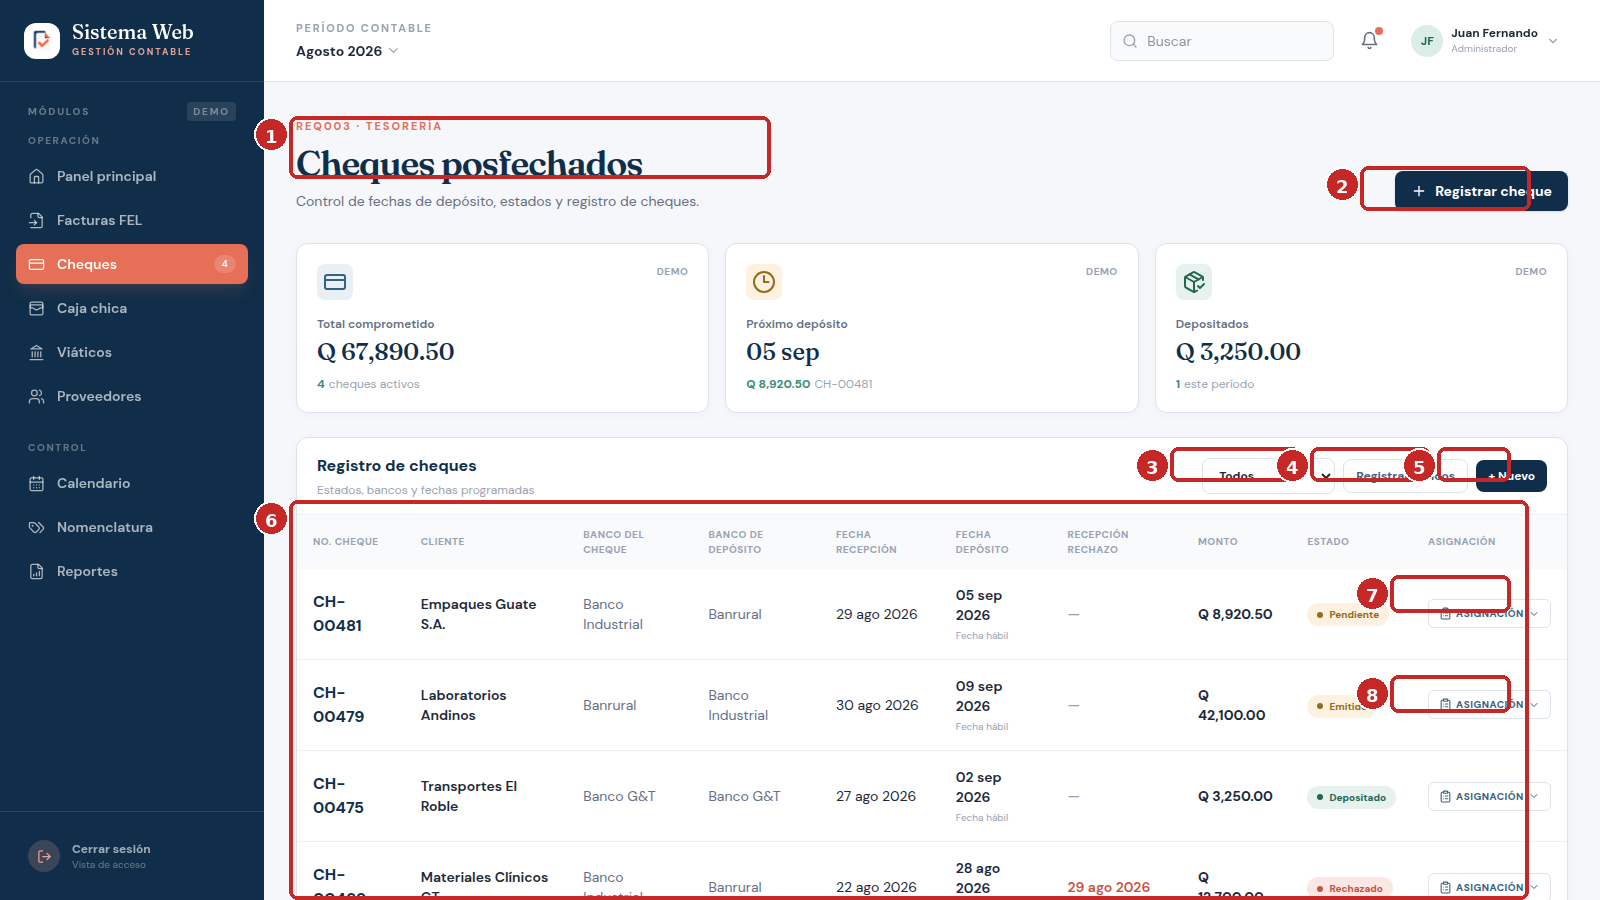
\includegraphics[width=0.92\linewidth]{capturas_reales/anotadas/pantalla_04_cheques_anotada.png}
    \caption*{Nota. Elaboración propia a partir del prototipo funcional.}
\end{figure}

\begin{enumerate}
\item Revise el resumen de compromisos, próximo depósito y cheques depositados.
\item Filtre la tabla por estado mediante la lista desplegable.
\item Haga clic en ``Registrar bancos'' para mantener los bancos disponibles.
\item Haga clic en ``Nuevo'' para registrar un cheque.
\item Revise la tabla con número de cheque, cliente, banco del cheque, banco de depósito, fecha de recepción, fecha de depósito, recepción de rechazo, monto y estado.
\item Haga clic en ``Asignación'' en el cheque que desea consultar.
\item Revise la fecha de factura, número de factura, visitador, número de recibo y días vencidos.
\item Repita la consulta para otro cheque cuando necesite comparar sus datos antes de registrar o dar seguimiento.
\end{enumerate}

\subsubsection{Caja chica}
Caja chica permite llamar una factura FEL por número, registrar recibos u otros documentos, asignar la cuenta contable y preparar la partida.

\begin{figure}[H]
    \centering
    \caption{Módulo de Caja chica con anotaciones numeradas.}
    \label{fig:manual_usuario_pantalla_05_caja_chica_anotada}
    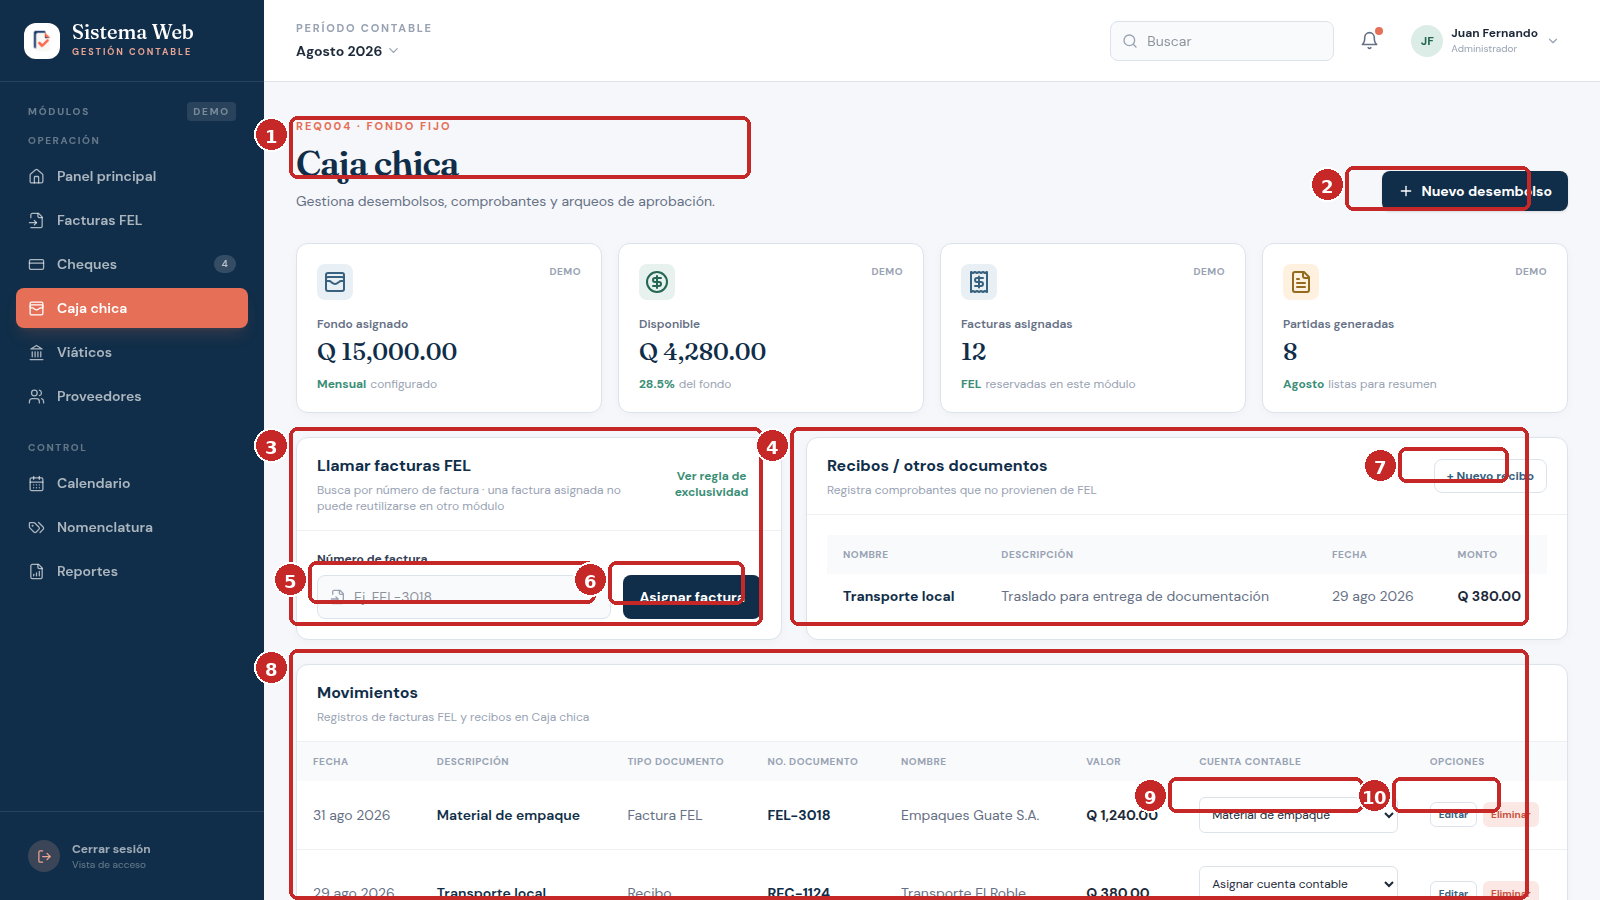
\includegraphics[width=0.92\linewidth]{capturas_reales/anotadas/pantalla_05_caja_chica_anotada.png}
    \caption*{Nota. Elaboración propia a partir del prototipo funcional.}
\end{figure}

\begin{enumerate}
\item revise el fondo asignado, disponible, facturas asignadas y partidas generadas.
\item escriba el número de factura FEL y presione ``Asignar factura''.
\item presione ``Nuevo recibo'' para registrar un documento que no proviene de FEL.
\item complete la fecha, descripción, tipo de documento, número, nombre y valor del movimiento.
\item revise la cuenta contable sugerida para el movimiento.
\item cuando la cuenta no sea reconocida, seleccione manualmente una cuenta registrada en Nomenclatura.
\item use ``Editar'' para corregir la descripción o los datos del movimiento y ``Eliminar'' solamente con autorización.
\item revise la tabla de Movimientos antes de generar la partida.
\item verifique los importes del Debe y las cuentas de gasto e IVA.
\item revise la contrapartida en el Haber y presione ``Imprimir resumen'' para preparar el documento.
\end{enumerate}

\subsubsection{Viáticos}
Viáticos administra colaboradores, territorios, giras, categorías de gasto y partidas automáticas.

\begin{figure}[H]
    \centering
    \caption{Módulo de Viáticos con anotaciones numeradas.}
    \label{fig:manual_usuario_pantalla_06_viaticos_anotada}
    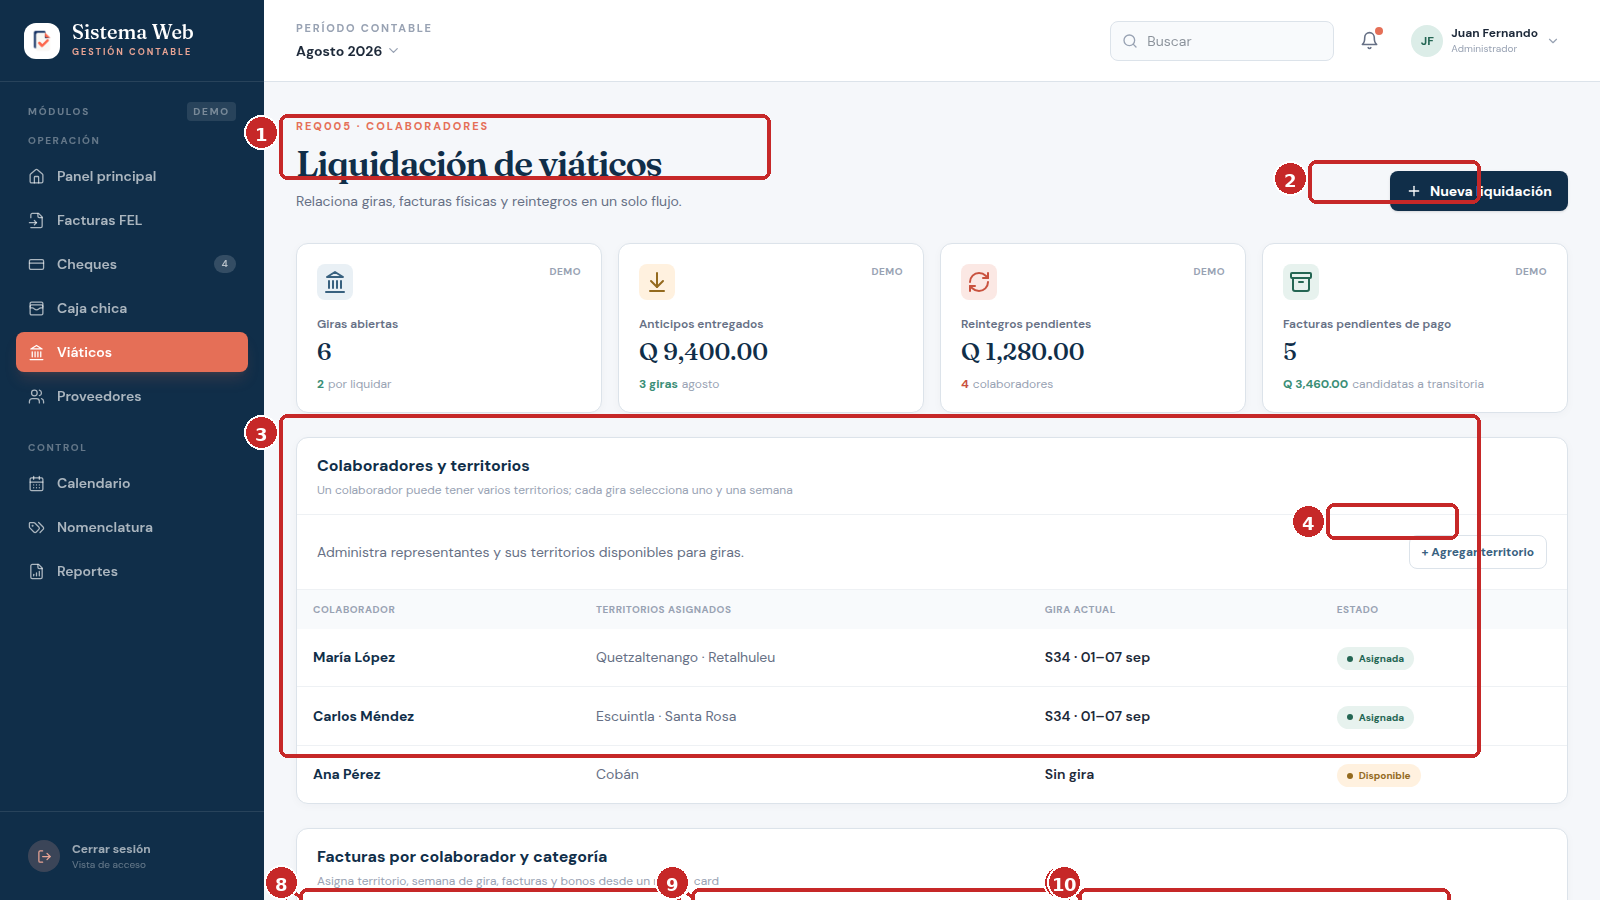
\includegraphics[width=0.92\linewidth]{capturas_reales/anotadas/pantalla_06_viaticos_anotada.png}
    \caption*{Nota. Elaboración propia a partir del prototipo funcional.}
\end{figure}

\begin{enumerate}
\item Revise las giras abiertas, anticipos, reintegros y facturas pendientes de pago.
\item Haga clic en ``Agregar territorio'' cuando deba asociar un territorio a un colaborador.
\item Seleccione el colaborador, el territorio y la semana de gira.
\item Seleccione la categoría ``Viáticos'', ``Movilidad'' o ``Actividades'' y haga clic en ``Asignar facturas''.
\item Recuerde que Movilidad está disponible durante la primera semana del mes según la regla del sistema.
\item Registre bonos u otros gastos indicando nombre, descripción y monto.
\item Revise la partida semanal y haga clic en ``Generar partida semanal''.
\item Haga clic en ``Generar cuenta transitoria'' para agrupar facturas pendientes de pago.
\end{enumerate}

\subsubsection{Asignación de facturas}
Esta pantalla permite vincular una factura con un colaborador, una gira, una categoría y una cuenta contable.

\begin{figure}[H]
    \centering
    \caption{Pantalla de asignación de facturas con anotaciones numeradas.}
    \label{fig:manual_usuario_pantalla_07_asignacion_facturas_anotada}
    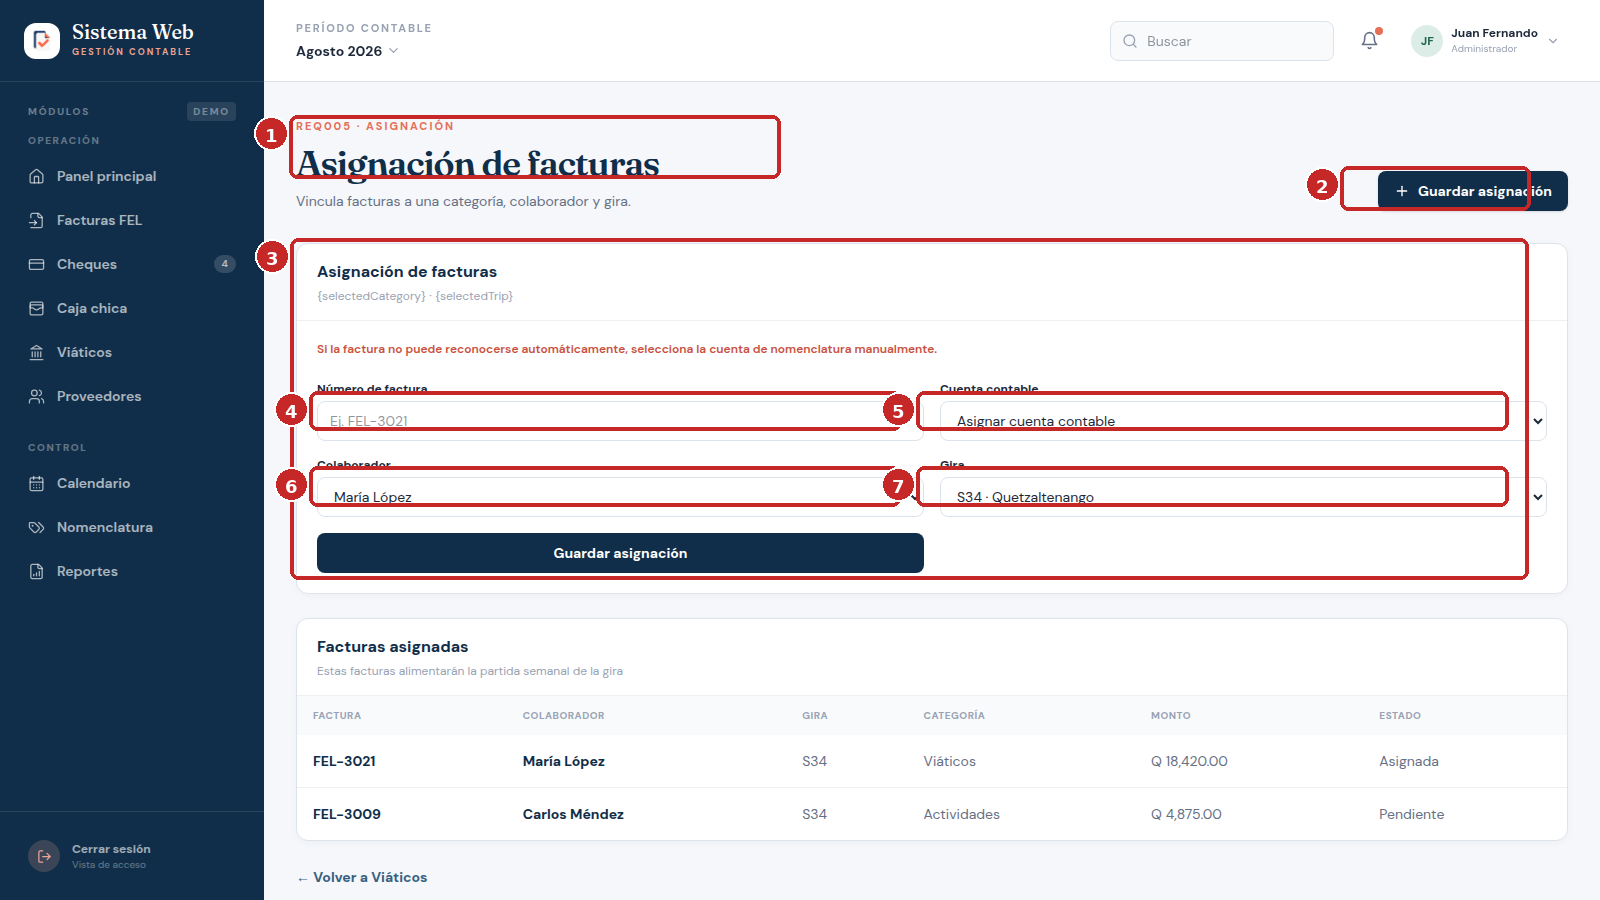
\includegraphics[width=0.92\linewidth]{capturas_reales/anotadas/pantalla_07_asignacion_facturas_anotada.png}
    \caption*{Nota. Elaboración propia a partir del prototipo funcional.}
\end{figure}

\begin{enumerate}
\item confirme la categoría y la gira seleccionadas.
\item escriba el número de factura.
\item seleccione la cuenta contable. Si el sistema no la reconoce, elija una cuenta registrada en Nomenclatura.
\item seleccione el colaborador.
\item seleccione la gira o territorio correspondiente.
\item presione ``Guardar asignación''.
\item confirme que la factura aparezca en la tabla de facturas asignadas con su estado correcto.
\end{enumerate}

\subsubsection{Proveedores}
Proveedores administra el registro por NIT, las condiciones de crédito, las retenciones, la cartera y las partidas.

\begin{figure}[H]
    \centering
    \caption{Módulo de Proveedores con anotaciones numeradas.}
    \label{fig:manual_usuario_pantalla_08_proveedores_anotada}
    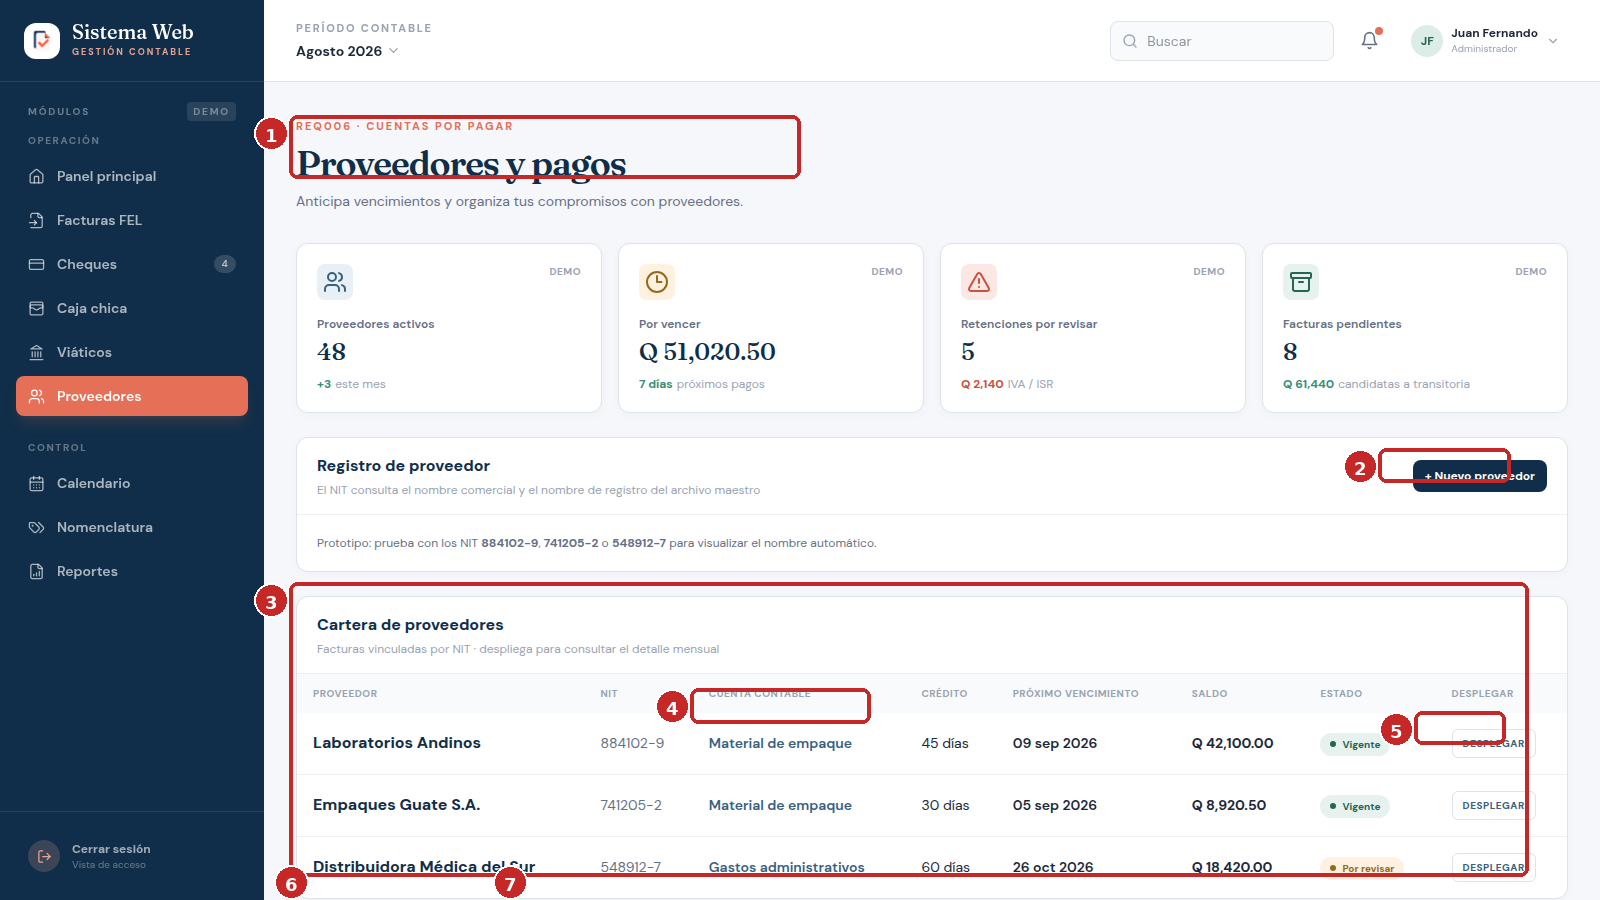
\includegraphics[width=0.92\linewidth]{capturas_reales/anotadas/pantalla_08_proveedores_anotada.png}
    \caption*{Nota. Elaboración propia a partir del prototipo funcional.}
\end{figure}

\begin{enumerate}
\item presione ``Nuevo proveedor'' para iniciar el registro.
\item escriba el NIT. El sistema consultará el nombre comercial y el nombre de registro disponibles.
\item revise la cartera con proveedor, NIT, cuenta contable, crédito, vencimiento, saldo y estado.
\item confirme la cuenta de Nomenclatura asociada al proveedor.
\item presione ``Desplegar'' para consultar las facturas mensuales.
\item presione ``Generar partida dentro del mes'' para obligaciones pagaderas en el período.
\item presione ``Generar partida transitoria'' para facturas pendientes de pago.
\end{enumerate}

\subsubsection{Calendario operativo}
Calendario presenta depósitos, pagos, cheques, giras y otras actividades por período.

\begin{figure}[H]
    \centering
    \caption{Módulo de Calendario con anotaciones numeradas.}
    \label{fig:manual_usuario_pantalla_09_calendario_anotada}
    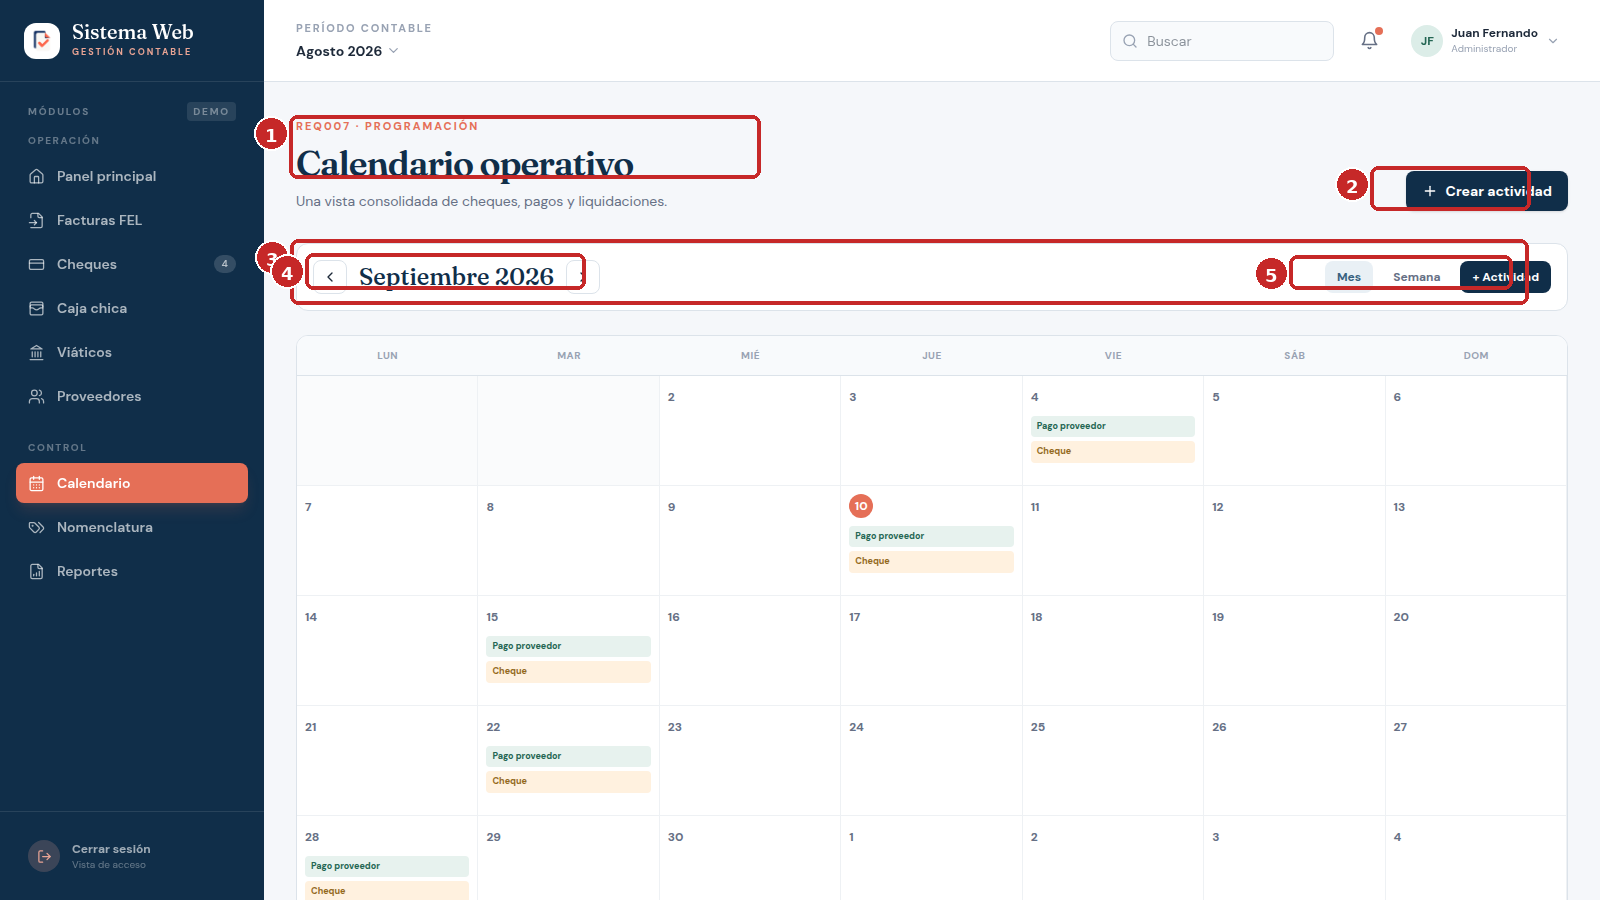
\includegraphics[width=0.92\linewidth]{capturas_reales/anotadas/pantalla_09_calendario_anotada.png}
    \caption*{Nota. Elaboración propia a partir del prototipo funcional.}
\end{figure}

\begin{enumerate}
\item revise el mes y año mostrados.
\item utilice las flechas para cambiar de período.
\item presione ``Mes'' para conservar la vista mensual.
\item consulte los eventos ubicados en cada fecha, como ``Pago proveedor'' y ``Cheque''.
\item presione ``Actividad'' para registrar una nueva actividad cuando tenga autorización.
\end{enumerate}

\subsubsection{Nomenclatura contable}
Nomenclatura contiene las cuentas que alimentan las sugerencias y partidas del sistema.

\begin{figure}[H]
    \centering
    \caption{Módulo de Nomenclatura con anotaciones numeradas.}
    \label{fig:manual_usuario_pantalla_10_nomenclatura_anotada}
    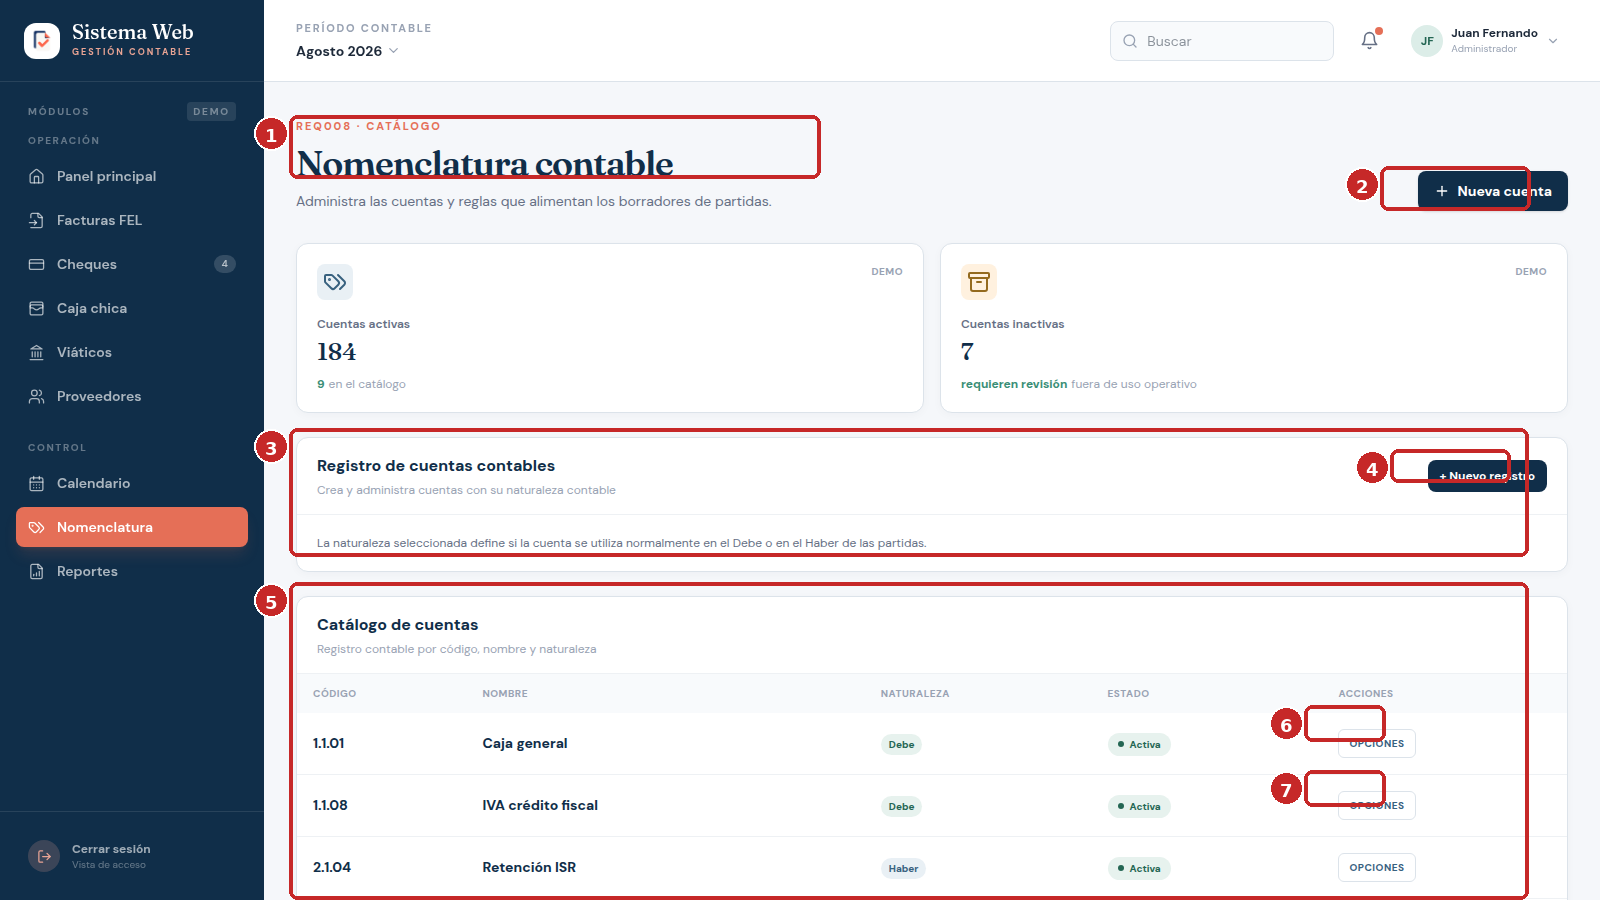
\includegraphics[width=0.92\linewidth]{capturas_reales/anotadas/pantalla_10_nomenclatura_anotada.png}
    \caption*{Nota. Elaboración propia a partir del prototipo funcional.}
\end{figure}

\begin{enumerate}
\item presione ``Nueva cuenta'' cuando corresponda crear una cuenta.
\item presione ``Nuevo registro'' para abrir el formulario de cuenta.
\item escriba código y nombre y seleccione la naturaleza Debe o Haber.
\item guarde el registro y verifique que la cuenta aparezca en el catálogo.
\item consulte el código, nombre, naturaleza y estado de cada cuenta.
\item abra ``Opciones'' para administrar el registro según sus permisos.
\end{enumerate}

\subsubsection{Reportes}
Reportes permite seleccionar el tipo de información, el período y los filtros para obtener indicadores.

\begin{figure}[H]
    \centering
    \caption{Módulo de Reportes con anotaciones numeradas.}
    \label{fig:manual_usuario_pantalla_11_reportes_anotada}
    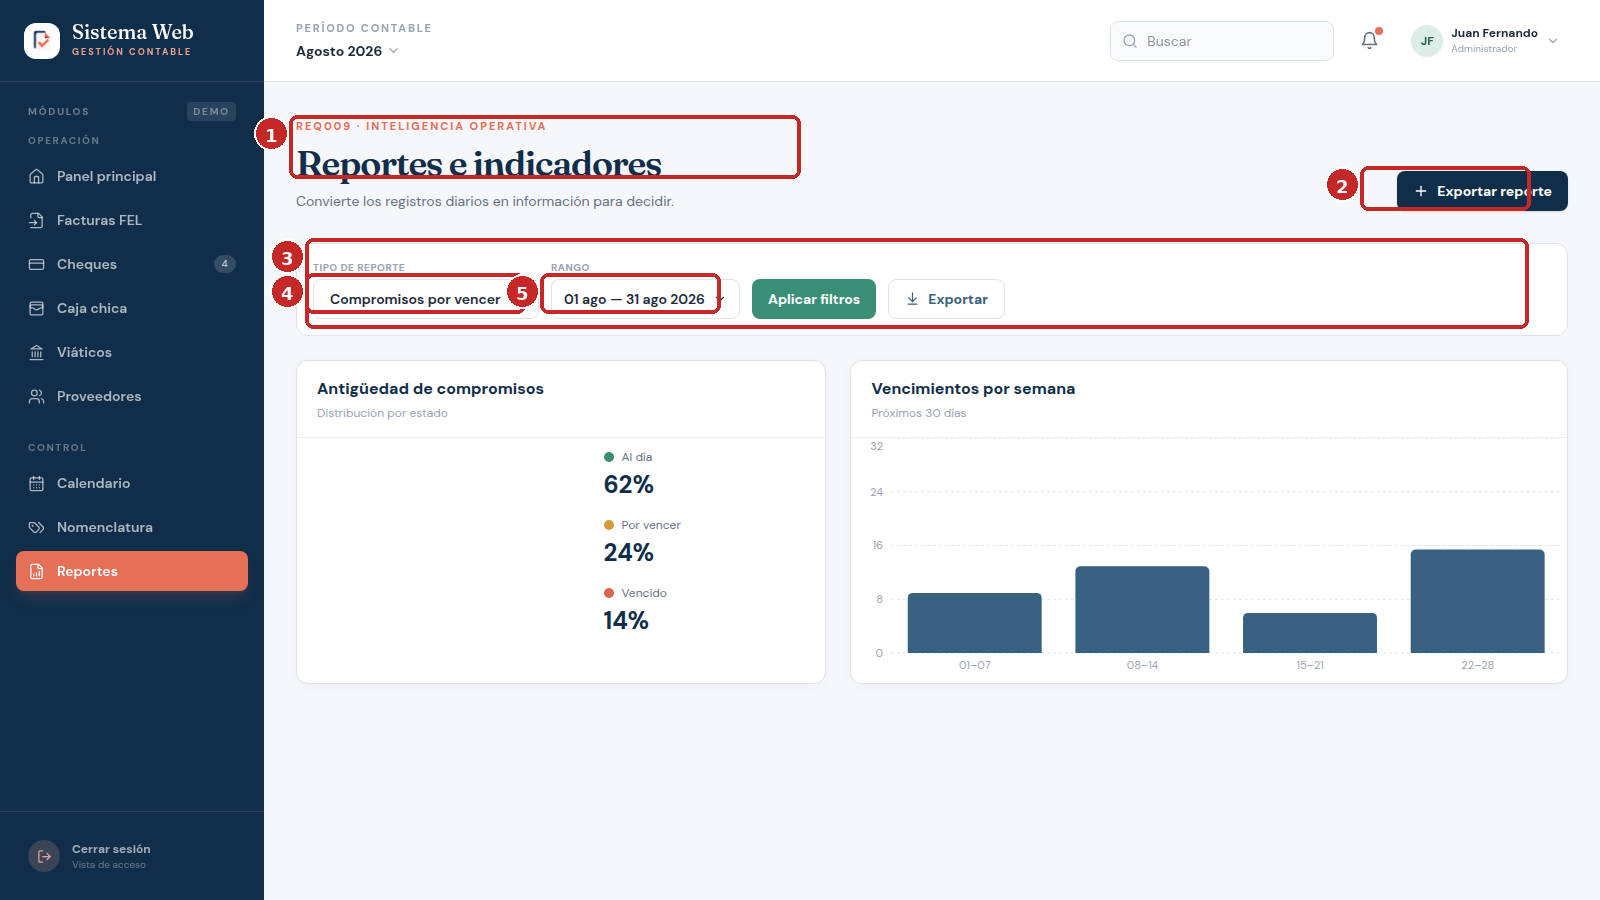
\includegraphics[width=0.92\linewidth]{capturas_reales/anotadas/pantalla_11_reportes_anotada.png}
    \caption*{Nota. Elaboración propia a partir del prototipo funcional.}
\end{figure}

\begin{enumerate}
\item confirme que se encuentra en ``Reportes e indicadores''.
\item seleccione el tipo de reporte.
\item seleccione el rango de fechas.
\item presione ``Aplicar filtros''.
\item presione ``Exportar'' para descargar o preparar el reporte autorizado.
\end{enumerate}

\subsubsection{Resumen de Caja chica}
El resumen presenta los movimientos que se imprimirán o archivarán.

\begin{figure}[H]
    \centering
    \caption{Resumen de Caja chica con anotaciones numeradas.}
    \label{fig:manual_usuario_pantalla_12_resumen_caja_anotada}
    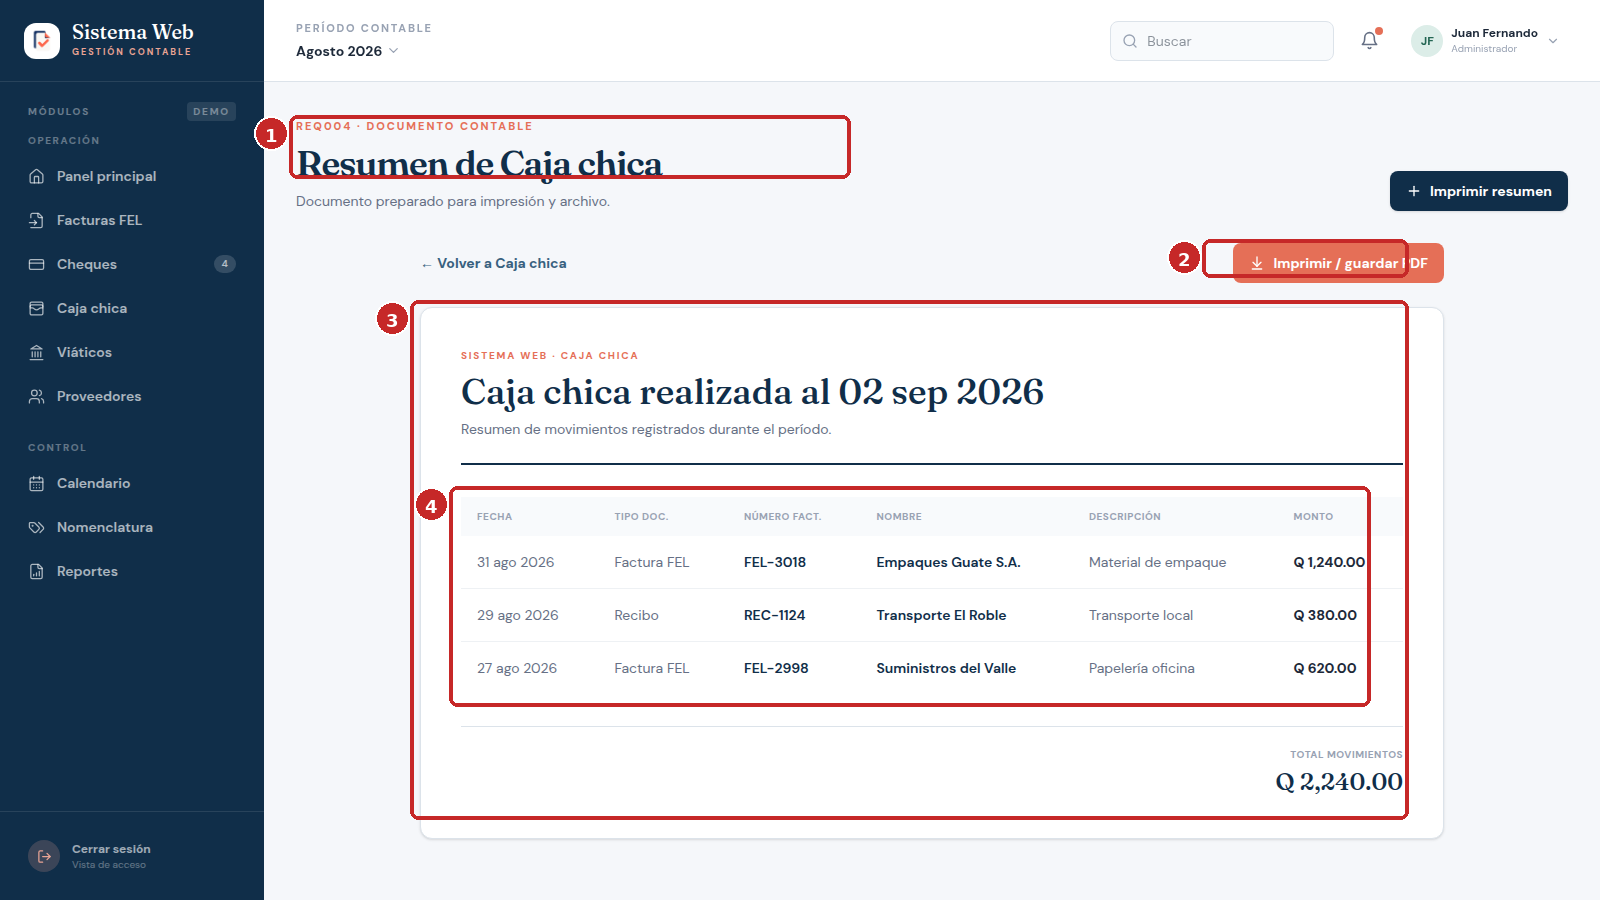
\includegraphics[width=0.92\linewidth]{capturas_reales/anotadas/pantalla_12_resumen_caja_anotada.png}
    \caption*{Nota. Elaboración propia a partir del prototipo funcional.}
\end{figure}

\begin{enumerate}
\item confirme el título y la fecha del resumen.
\item presione ``Imprimir / guardar PDF''.
\item verifique que el documento incluya fecha, tipo de documento, número, nombre, descripción y monto.
\item revise el total de movimientos antes de imprimir o guardar el archivo.
\end{enumerate}

\subsubsection{Mensajes de error y solución}
Cuando las credenciales sean rechazadas, vuelva a escribir el usuario y la contraseña. Si una factura no puede clasificarse, asígnele manualmente una cuenta de Nomenclatura. Si falta un dato obligatorio, complete el campo señalado antes de guardar. Si una partida no cuadra, revise Debe, Haber, IVA, retenciones y descuentos. Si la pantalla no carga, actualice el navegador y comuníquese con soporte si el problema persiste.

\subsubsection{Recomendaciones de seguridad}
Mantenga sus credenciales bajo resguardo, cierre sesión al terminar, revise los documentos antes de aprobarlos y no elimine información sin autorización. Verifique siempre que la cuenta contable corresponda al gasto y que la operación se registre en el período correcto.

\subsubsection{Flujo recomendado de trabajo}
Para mantener la trazabilidad contable, inicie el período revisando el Panel principal, importe las facturas FEL/SAT, verifique los cheques y registre las operaciones de Caja chica. Posteriormente, asigne las facturas de viáticos, actualice la cartera de proveedores, revise el Calendario y genere los reportes autorizados.

\subsubsection{Cierre de operaciones}
Antes de cerrar el período, confirme que las facturas tengan una cuenta de Nomenclatura, que las partidas estén cuadradas, que los cheques tengan el estado correcto y que las facturas pendientes se encuentren identificadas como partidas transitorias. Guarde los reportes autorizados según las políticas internas.

\subsubsection{Glosario básico}
\begin{description}
\item[FEL/SAT] Factura electrónica y documentos tributarios consultados o importados desde la información del SAT.
\item[Nomenclatura] Catálogo de cuentas contables utilizado para clasificar gastos y construir partidas.
\item[Partida transitoria] Registro contable temporal utilizado cuando una factura está pendiente de pago.
\item[Viático] Gasto asociado a una gira, colaborador, territorio y semana de trabajo.
\item[Arqueo o resumen] Documento de revisión de movimientos y saldo de Caja chica.
\end{description}

\subsubsection{Seguimiento y trazabilidad de operaciones}
Cada registro debe revisarse antes de continuar con el siguiente paso. Cuando una operación genere una partida, una asignación o un cambio de estado, conserve el número de documento, la fecha y el módulo en el que se realizó. Esta información facilita la revisión posterior y permite comunicar una incidencia con datos verificables.

\subsubsection{Criterios de revisión antes del cierre}
Antes de finalizar la jornada o el período, confirme que las operaciones guardadas correspondan al período correcto, que no existan documentos duplicados y que las cuentas contables utilizadas estén activas. Cuando el sistema solicite una asignación manual, seleccione la cuenta que corresponda al gasto y solicite una segunda revisión si la operación afecta una partida contable.

\subsubsection{Atención de incidencias}
Cuando una operación no produzca el resultado esperado, registre la fecha, el módulo, la acción realizada y el mensaje mostrado. Evite repetir una importación o un registro hasta confirmar que la primera operación no fue guardada. El reporte debe remitirse al responsable designado sin incluir contraseñas, tokens ni información que no sea necesaria para diagnosticar el problema.
\clearpage
\setcounter{figure}{0}
\setcounter{table}{0}
% Manual Técnico del Sistema Web de gestión contable.
% Este archivo se incorpora directamente desde main.tex como Apéndice B.
% Arquitectura declarada: Angular, Python y PostgreSQL.
\newpage

\section{Manual Técnico}\label{ap:manual_tecnico}
\begin{center}
\vspace*{2cm}
{\Large\textbf{APÉNDICE B}}\par
\vspace{1.5cm}
{\Large\textbf{MANUAL TÉCNICO}}\par
\vspace{0.8cm}
{\large Sistema Web de gestión contable}\par
\vspace{2cm}
\begin{minipage}{0.82\textwidth}
\centering
Descripción técnica de la arquitectura, configuración, base de datos, seguridad, mantenimiento y pruebas del sistema.
\end{minipage}
\vfill
Documento complementario del trabajo de graduación\par
\end{center}

\newpage
\setlength{\parindent}{1.27cm}
\setlength{\parskip}{0pt}
\setstretch{2.0}

\subsubsection{Introducción}
Este manual documenta la construcción, configuración, despliegue y mantenimiento del Sistema Web de gestión contable. Está dirigido al personal técnico, desarrolladores y responsables de soporte.

\subsubsection{Propósito y alcance}
Este manual describe la arquitectura, configuración, base de datos, seguridad, operación y mantenimiento del Sistema Web de gestión contable. Está dirigido al personal técnico, desarrolladores y responsables de soporte. La documentación se rige por las especificaciones de la tesis: \textbf{Angular} para el frontend, \textbf{Python} para el backend y \textbf{PostgreSQL} para la persistencia de datos.

El sistema administra comprobantes FEL/SAT, cheques posfechados, Caja chica, Viáticos, Proveedores, Calendario, Nomenclatura y Reportes. La interfaz debe conservar la distribución visual mostrada en las capturas reales del prototipo y las reglas de negocio descritas en el Capítulo III.

\subsubsection{Arquitectura general}
La solución se organiza en tres capas. La Capa de Presentación se implementa como una aplicación SPA con Angular, Angular Router, formularios reactivos y componentes de Angular Material. La Capa de Lógica de Negocio se implementa en Python mediante una API REST, preferentemente con FastAPI, Pydantic y SQLAlchemy. La Capa de Persistencia utiliza PostgreSQL con restricciones, índices, llaves primarias y llaves foráneas.

El frontend se comunica con el backend mediante HTTPS y cargas JSON. El backend valida permisos, ejecuta reglas contables, registra auditoría y consulta PostgreSQL. Los archivos XML o Excel de FEL/SAT deben validarse en el servidor antes de almacenarse o procesarse. Las credenciales no deben guardarse en el navegador ni incluirse en el código fuente.

\begin{figure}[H]
    \centering
    \caption{Arquitectura lógica del Sistema Web.}
    \label{fig:manual_tecnico_arquitectura}
    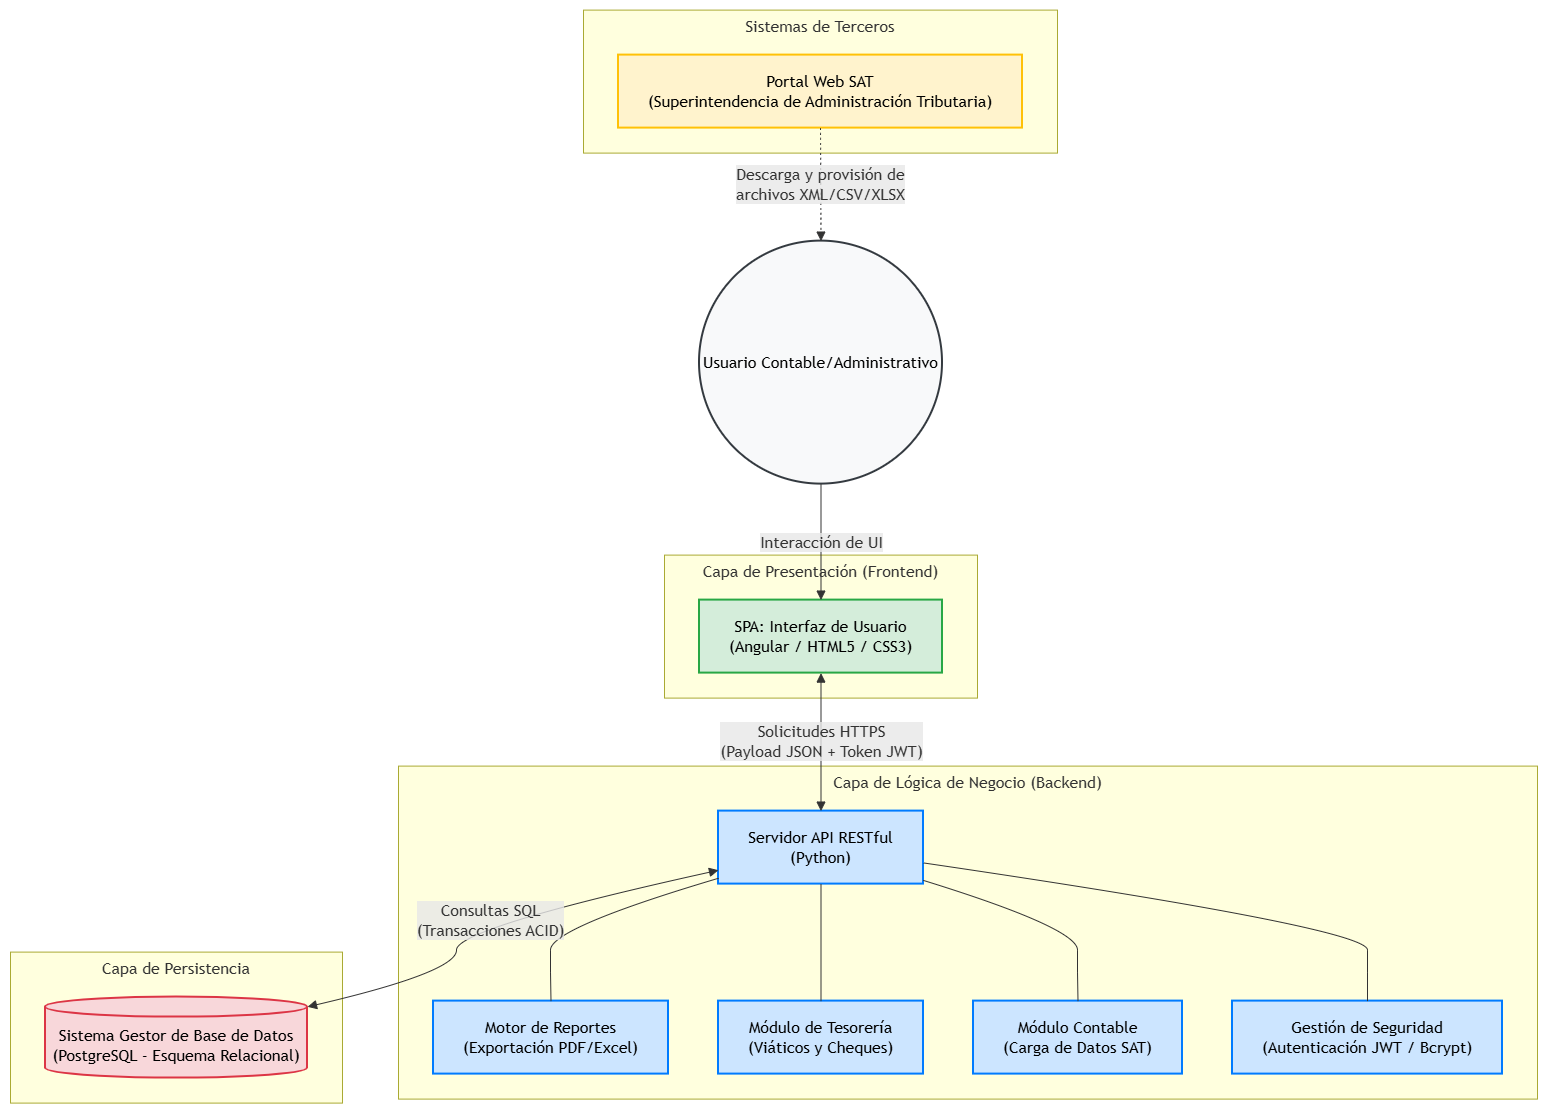
\includegraphics[width=0.92\linewidth]{imagenes/Arquitectura.png}
    \caption*{Nota. Elaboración propia con base en la arquitectura definida para el proyecto.}
\end{figure}

\subsubsection{Módulos funcionales}

\begin{longtable}{p{0.24\linewidth}p{0.68\linewidth}}
\textbf{Módulo} & \textbf{Responsabilidad técnica} \\
Login & Autenticar al usuario, emitir el token de sesión y aplicar permisos por rol. \\
Facturas FEL/SAT & Recibir XML o Excel, validar estructura, detectar duplicados, guardar comprobantes y permitir clasificación contable. \\
Cheques & Registrar cliente, bancos, fechas, estado, recepción de rechazo y asignación de factura. \\
Caja chica & Llamar facturas FEL por número, registrar recibos, controlar movimientos, aplicar nomenclatura y generar partidas. \\
Viáticos & Administrar colaboradores, territorios, giras, semanas, categorías, facturas, bonos y partidas semanales o transitorias. \\
Proveedores & Registrar NIT, crédito, retenciones, descuentos, cartera y partidas dentro del mes o transitorias. \\
Calendario & Consultar vencimientos, pagos, depósitos, cheques, giras y actividades. \\
Nomenclatura & Administrar código, nombre, naturaleza y estado de las cuentas contables. \\
Reportes & Consultar indicadores, filtros por período y exportaciones autorizadas. \\
\end{longtable}

\subsubsection{Diseño de la base de datos}
El modelo debe separar catálogos, documentos operativos y resultados contables. Las entidades principales son \texttt{usuarios}, \texttt{roles}, \texttt{permisos}, \texttt{proveedores}, \texttt{colaboradores}, \texttt{territorios}, \texttt{cuentas\_contables}, \texttt{bancos}, \texttt{facturas}, \texttt{cheques}, \texttt{movimientos\_caja\_chica}, \texttt{recibos}, \texttt{giras}, \texttt{liquidaciones\_viaticos}, \texttt{asignaciones\_facturas}, \texttt{partidas\_contables}, \texttt{detalles\_partida} y \texttt{auditoria\_eventos}.

Proveedor se relaciona con Factura y puede tener una cuenta contable asociada. Una Factura puede asignarse exclusivamente a Caja chica o Viáticos. Cheque se relaciona con Cliente, bancos, factura y recibo. Colaborador puede tener varios Territorios y una Gira selecciona un territorio y una semana. Partida contable contiene múltiples Detalles de partida, cada uno con cuenta, naturaleza, Debe y Haber.

Las tablas deben utilizar identificadores UUID o enteros autogenerados, fechas con zona horaria cuando corresponda, campos monetarios con tipo NUMERIC(14,2), estados controlados y restricciones de integridad. Las operaciones de generación de partidas deben ejecutarse dentro de transacciones PostgreSQL y verificar que el total del Debe sea igual al total del Haber.

\begin{figure}[H]
    \centering
    \caption{Modelo de base de datos PostgreSQL.}
    \label{fig:manual_tecnico_diagramabd}
    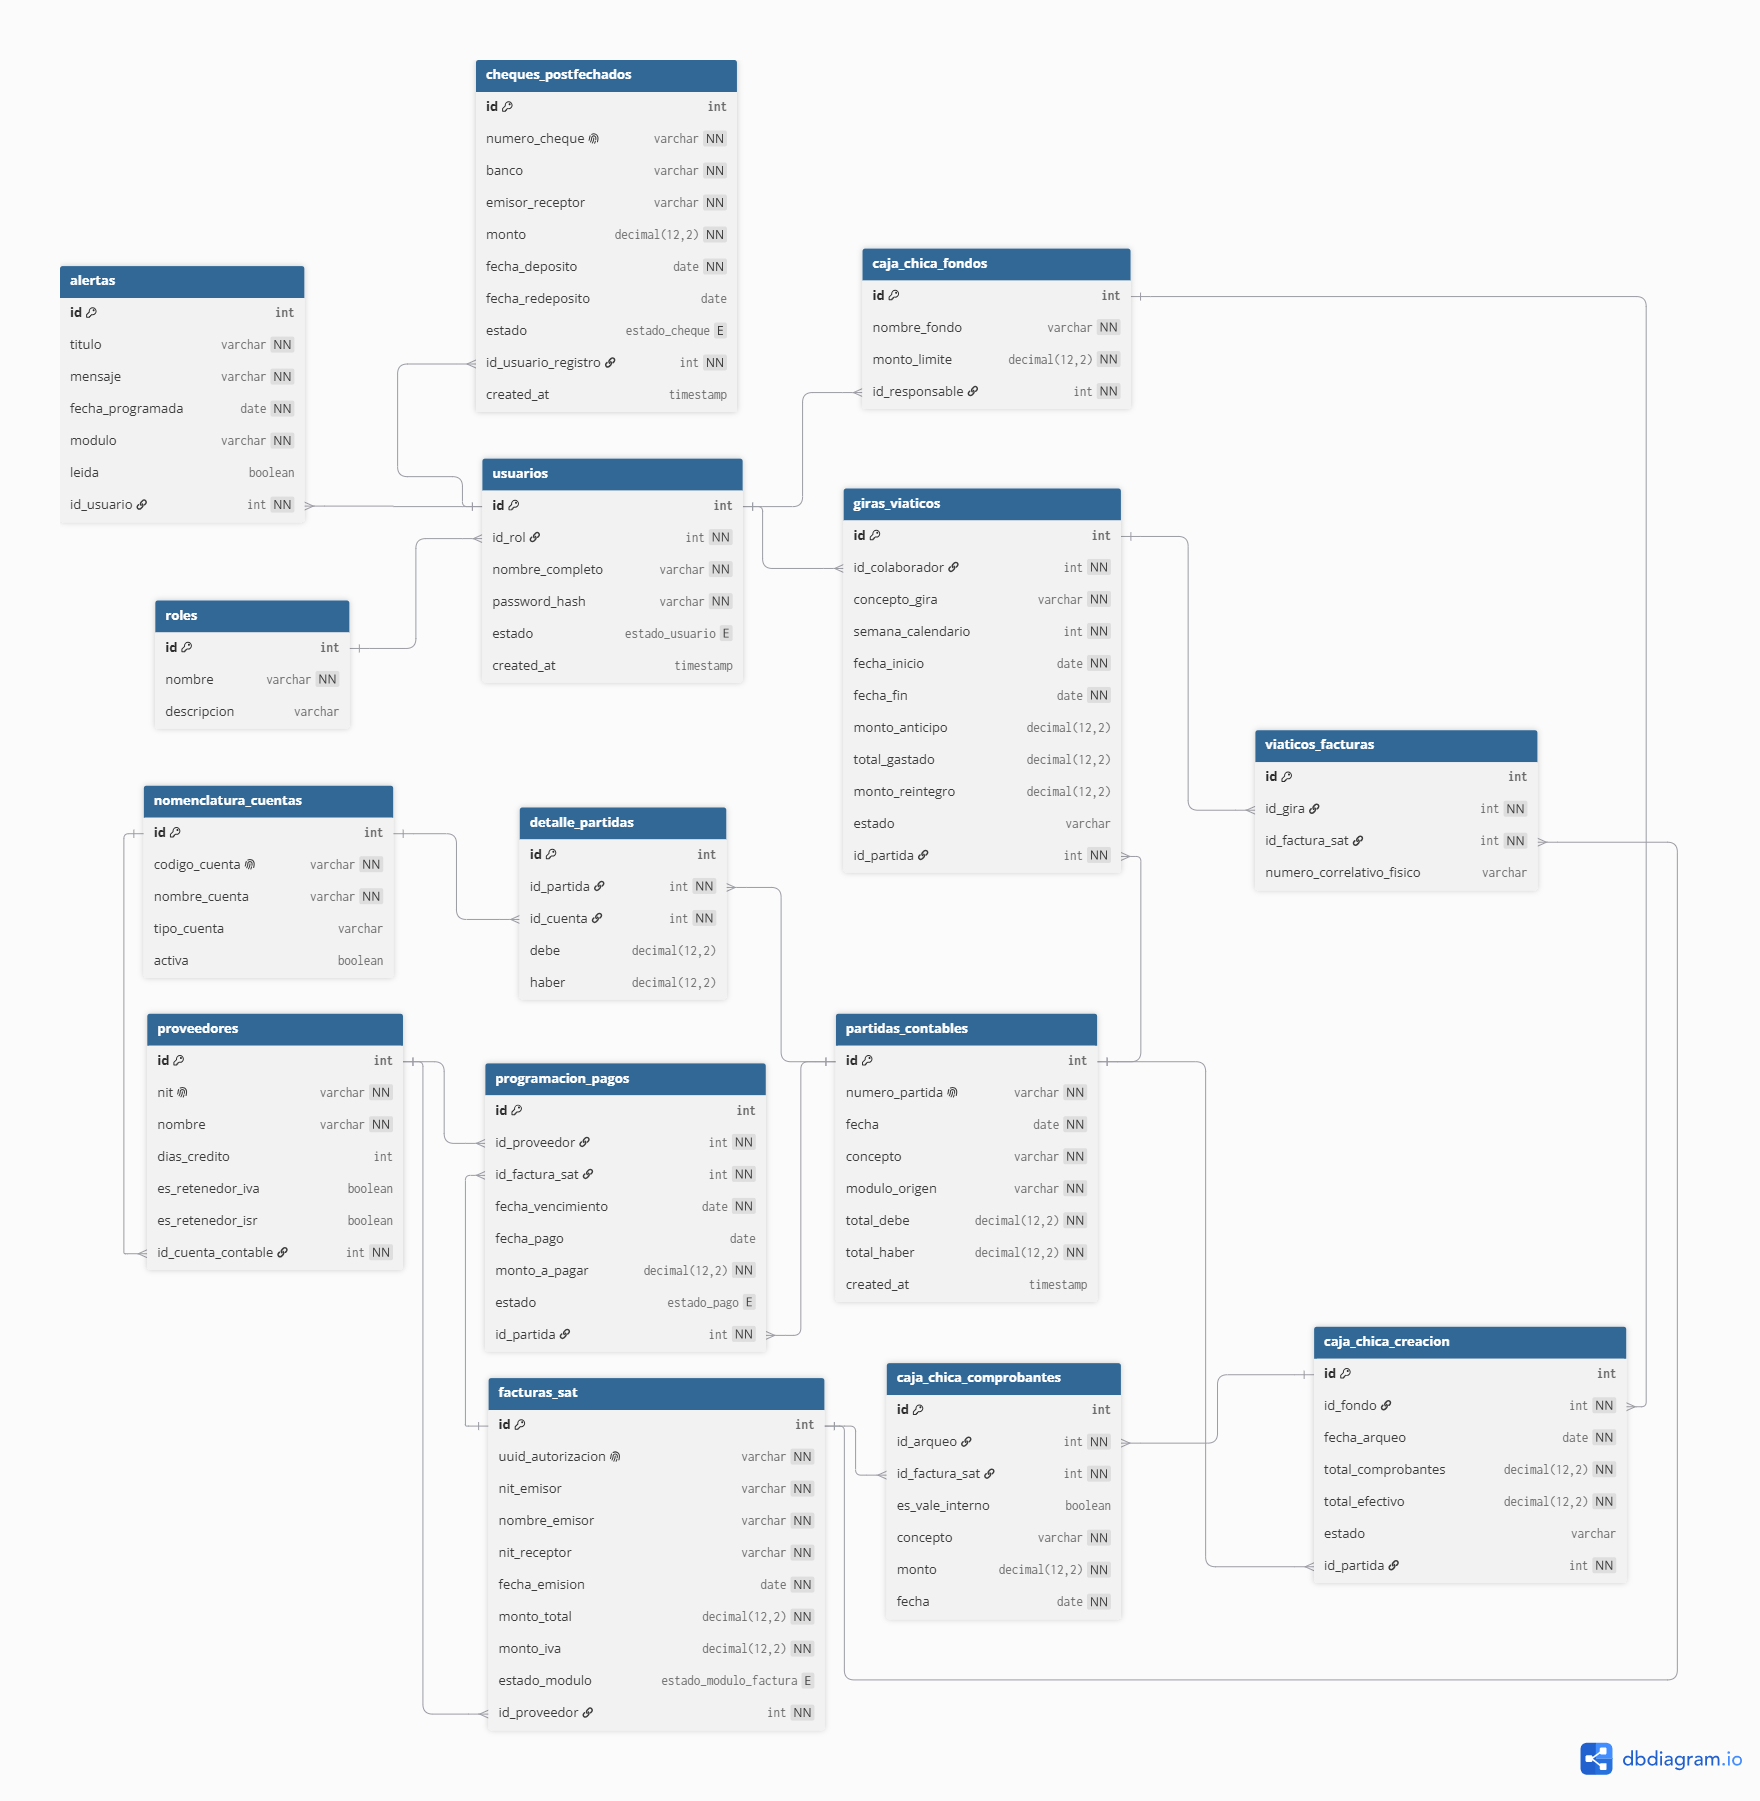
\includegraphics[width=0.92\linewidth]{imagenes/diagramabd.png}
    \caption*{Nota. Elaboración propia para el diseño de persistencia del Sistema Web.}
\end{figure}

\subsubsection{Reglas contables y de integridad}
La cuenta asignada al proveedor debe estar registrada en Nomenclatura. Cuando el sistema no reconoce automáticamente una factura por su descripción, combustible, lugar o concepto, el usuario debe seleccionar una cuenta contable válida del catálogo. La misma regla se aplica a Caja chica y Viáticos.

La generación dentro del mes utiliza Bancos como contrapartida cuando corresponde al pago del período. La partida transitoria utiliza Cuenta transitoria para documentos pendientes de pago. Retención ISR, Retención IVA y Otros descuentos deben conservarse como líneas independientes en el Haber. Las facturas ya asignadas no deben reutilizarse en otro módulo sin una operación autorizada de reversión.

\subsubsection{Tecnologías utilizadas}
La solución utiliza Angular para el frontend, Python para el backend y PostgreSQL para la persistencia. Angular organiza la interfaz como una aplicación de una sola página; Python expone la API y concentra la lógica de negocio; PostgreSQL mantiene la integridad, trazabilidad y consistencia de los datos contables. Las dependencias y versiones exactas deben mantenerse documentadas en los archivos de configuración del proyecto.

\subsubsection{Estructura del proyecto}

\begin{verbatim}
frontend-angular/
  src/app/
    core/                 # autenticación, guards e interceptores
    shared/               # componentes, pipes y validadores
    layout/               # menú lateral y barra superior
    modules/
      login/
      facturas-fel/
      cheques/
      caja-chica/
      viaticos/
      proveedores/
      calendario/
      nomenclatura/
      reportes/
    app-routing.module.ts

backend-python/
  app/
    api/                  # routers REST
    core/                 # configuración y seguridad
    models/               # modelos SQLAlchemy
    schemas/              # esquemas Pydantic
    services/             # reglas de negocio
    repositories/         # acceso a PostgreSQL
    migrations/           # Alembic
    main.py

base-datos/
  migrations/
  seeds_controlados/

documentacion/
  manuales/
  capitulos/
\end{verbatim}

\subsubsection{API y autenticación}
Los endpoints deben versionarse, por ejemplo, bajo \texttt{/api/v1}. El inicio de sesión devuelve un token JWT de corta duración y el frontend lo envía mediante un interceptor HTTP. Los guards de Angular restringen rutas y el backend vuelve a validar el rol; nunca se debe confiar únicamente en las restricciones de la interfaz.

Los endpoints deben validar tipos, campos obligatorios, permisos y estados de negocio. Las respuestas deben utilizar códigos HTTP coherentes, mensajes sin información sensible y un identificador de correlación para facilitar el diagnóstico. Las cargas de archivos deben limitar tamaño, extensión y contenido, y deben analizarse antes de procesarse.

\subsubsection{Configuración del entorno}
Para desarrollo se requiere Python 3.11 o la versión institucional aprobada, Node.js compatible con Angular, PostgreSQL, un entorno virtual de Python y las dependencias del proyecto. Las variables de entorno deben incluir la URL de PostgreSQL, secreto JWT, duración del token, configuración CORS y parámetros de almacenamiento.

Ejemplo de preparación del backend:

\begin{verbatim}
python -m venv .venv
source .venv/bin/activate
pip install -r requirements.txt
alembic upgrade head
uvicorn app.main:app --reload
\end{verbatim}

Ejemplo de preparación del frontend:

\begin{verbatim}
npm install
ng serve
ng build --configuration production
\end{verbatim}

Las claves y contraseñas deben permanecer fuera del repositorio. Para producción, el servidor debe usar HTTPS, variables protegidas y un usuario de PostgreSQL con los permisos mínimos necesarios.

\subsubsection{Despliegue}
El backend Python debe ejecutarse detrás de un servidor ASGI y un proxy inverso con HTTPS. El frontend Angular compilado debe publicarse como archivos estáticos o mediante el hosting institucional. Las rutas de Angular deben redirigir a \texttt{index.html}. PostgreSQL debe ubicarse en una red protegida, con respaldos automáticos, monitoreo y control de conexiones.

Antes de publicar se debe ejecutar una migración en un entorno de prueba, verificar login, importación FEL, asignación exclusiva, generación de partidas, exportación de reportes y recuperación ante errores. No se deben usar datos de demostración en el ambiente productivo.

\subsubsection{Mantenimiento preventivo y correctivo}
El mantenimiento preventivo incluye actualizar dependencias con control de versiones, revisar logs, aplicar migraciones, comprobar índices y validar respaldos. El mantenimiento correctivo debe reproducir el incidente, registrar módulo, usuario, fecha y operación, corregir la causa y ejecutar pruebas de regresión.

Los respaldos de PostgreSQL deben incluir al menos una copia completa y copias del esquema. Se debe comprobar periódicamente la restauración en un ambiente separado. Las operaciones destructivas sobre facturas, cheques, movimientos y partidas deben requerir autorización y conservar una entrada de auditoría.

\subsubsection{Evidencias visuales}
Las capturas incorporadas al paquete fueron tomadas del prototipo navegable y se conservan en la carpeta de imágenes. Las versiones anotadas del Manual de Usuario agregan números rojos y recuadros para explicar cada control. Las láminas agrupadas de componentes se mantienen como material complementario del Capítulo III.

\begin{figure}[H]
    \centering
    \caption{Componentes visuales agrupados del sistema.}
    \label{fig:manual_tecnico_elementos_04_tablas_tarjetas}
    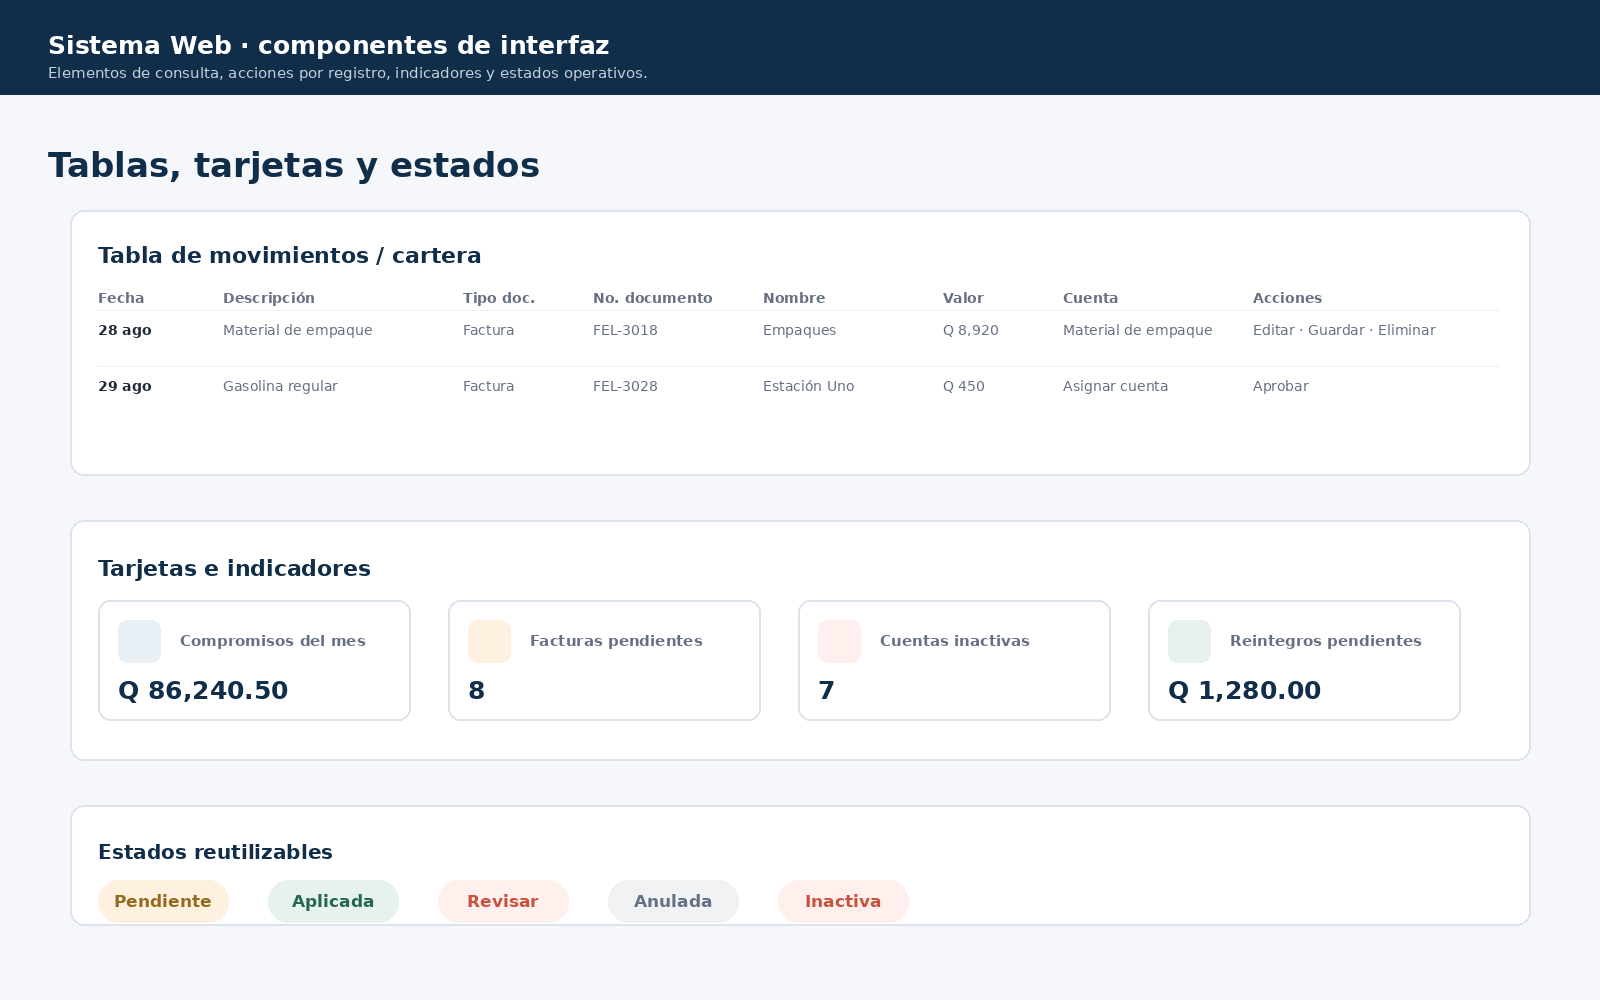
\includegraphics[width=0.92\linewidth]{imagenes/elementos_04_tablas_tarjetas.png}
    \caption*{Nota. Elaboración propia a partir de los componentes del prototipo.}
\end{figure}

\subsubsection{Matriz mínima de pruebas técnicas}

\begin{longtable}{p{0.25\linewidth}p{0.34\linewidth}p{0.29\linewidth}}
\textbf{Módulo} & \textbf{Prueba} & \textbf{Resultado esperado} \\
Login & Credenciales válidas e inválidas & Acceso autorizado o mensaje controlado. \\
FEL/SAT & XML duplicado o con error & Rechazo, aviso y conservación de trazabilidad. \\
Cheques & Cambio de estado y asignación & Estado, fechas y detalle de factura consistentes. \\
Caja chica & Movimiento sin cuenta reconocida & Solicitud de clasificación manual desde Nomenclatura. \\
Viáticos & Partida semanal y transitoria & Debe y Haber balanceados y documentos no duplicados. \\
Proveedores & Vencido y pendiente de pago & Selección correcta entre Bancos y Cuenta transitoria. \\
Nomenclatura & Cuenta Debe/Haber activa o inactiva & Validación de naturaleza y disponibilidad. \\
Reportes & Filtro y exportación & Información correspondiente al período seleccionado. \\
\end{longtable}


\subsubsection{Acceso e instalación}
La instalación se realiza en tres capas. Primero se prepara el entorno del frontend Angular y se instalan sus dependencias. Después se configura el servicio backend desarrollado en Python y sus variables de entorno. Finalmente se crea la base de datos PostgreSQL, se aplican las migraciones y se verifica la conexión entre las capas.

\subsubsection{Configuración por ambientes}
El proyecto debe separar los ambientes de desarrollo, pruebas y producción. Cada ambiente debe utilizar sus propias credenciales, URL de conexión y parámetros de seguridad. Las claves de acceso no deben almacenarse dentro del código fuente ni incorporarse al repositorio.

\subsubsection{Respaldo y recuperación}
El responsable técnico debe programar respaldos de PostgreSQL, verificar periódicamente que los archivos puedan restaurarse y documentar la fecha, responsable y resultado de cada prueba. Antes de una actualización, debe realizarse un respaldo completo y conservarse una copia fuera del servidor principal.

\subsubsection{Lista de verificación de mantenimiento}
El mantenimiento incluye actualizar dependencias de Angular y Python, revisar logs, verificar tareas programadas, comprobar el espacio disponible de PostgreSQL, validar permisos y ejecutar las pruebas funcionales de los módulos FEL/SAT, Cheques, Caja chica, Viáticos, Proveedores, Nomenclatura y Reportes.

\subsubsection{Pruebas técnicas mínimas}
\begin{longtable}{p{3.5cm}p{7.5cm}p{3cm}}
\caption{Pruebas técnicas mínimas del sistema}\label{tab:B_pruebas_tecnicas}\\
\toprule
\textbf{Prueba} & \textbf{Resultado esperado} & \textbf{Responsable}\\
\midrule
Conexión a PostgreSQL & El backend establece conexión y registra el resultado sin exponer credenciales. & Técnico\\
Autenticación & Angular envía la solicitud al backend Python y recibe una respuesta controlada. & Técnico\\
Importación FEL & El sistema valida el archivo y evita duplicados. & Auxiliar\\
Partida contable & Debe y Haber coinciden antes de guardar el registro. & Contador\\
Respaldo & La copia puede restaurarse en un ambiente de prueba. & Técnico\\
\bottomrule
\end{longtable}

\subsubsection{Anexos técnicos}
Los anexos técnicos comprenden el diagrama de arquitectura, el modelo de datos PostgreSQL, la matriz mínima de pruebas y las capturas de referencia del sistema. Estos anexos respaldan la explicación técnica y deben mantenerse sincronizados con los cambios aprobados en Angular, Python y PostgreSQL.

\clearpage
\setcounter{figure}{0}
\setcounter{table}{0}
